\documentclass[10pt,a4paper]{article}

% ---------------------------------------------------------------
% Pacotes
% ---------------------------------------------------------------
\usepackage[T1]{fontenc}
\usepackage[utf8]{inputenc}
\usepackage[portuguese]{babel}
\usepackage{lmodern}
\usepackage{setspace}
\usepackage[a4paper,top=2.2cm,bottom=2.2cm,left=2cm,right=2cm,headheight=14pt]{geometry}
\usepackage{xcolor}
\usepackage{graphicx}
\usepackage{amsmath,amssymb,bm}
\usepackage{booktabs}
\usepackage{array}
\usepackage[output-decimal-marker={,}]{siunitx}
\usepackage{enumitem}
\usepackage{fancyhdr}
\usepackage{lastpage}
\usepackage{titlesec}
\usepackage[font=small,labelfont={bf,color=istblue},skip=8pt]{caption}
\usepackage{float}
\usepackage{newfloat}
\DeclareFloatingEnvironment[name=Equação,placement=H]{equacao}
\newcommand{\formula}[3]{\begin{equacao}[H]\centering$\displaystyle #1$\caption{#2}\label{#3}\end{equacao}}
\usepackage[hidelinks]{hyperref}
\urlstyle{same}

% ---------------------------------------------------------------
% Cores e estilo
% ---------------------------------------------------------------
\definecolor{istblue}{RGB}{0,158,224}
\definecolor{istdark}{RGB}{31,45,61}
\definecolor{istgray}{RGB}{95,110,125}

\newcommand{\curso}{Desempenho e Dimensionamento de Redes e Sistemas}
\newcommand{\cursosigla}{DDRS}
\newcommand{\grupo}{Grupo 04}
\newcommand{\documento}{Laboratório 2}

\setlength{\parindent}{0pt}
\setlength{\parskip}{7pt plus 2pt}
\setstretch{1.15}
\setlength{\intextsep}{16pt plus 4pt minus 2pt}

\titleformat{\section}{\Large\bfseries\color{istdark}}{\thesection.}{0.5em}{}
\titleformat{\subsection}{\large\bfseries\color{istdark}}{\thesubsection.}{0.5em}{}
\titleformat{\subsubsection}{\normalsize\bfseries\color{istdark}}{\thesubsubsection.}{0.5em}{}
\titlespacing*{\section}{0pt}{22pt}{10pt}
\titlespacing*{\subsection}{0pt}{18pt}{8pt}
\titlespacing*{\subsubsection}{0pt}{14pt}{6pt}

\pagestyle{fancy}
\fancyhf{}
\fancyhead[L]{\scriptsize\color{istgray}\curso}
\fancyhead[R]{\scriptsize\color{istgray}\grupo\ $|$ \documento}
\fancyfoot[C]{\scriptsize\color{istgray}\thepage\ / \pageref{LastPage}}
\renewcommand{\headrulewidth}{0.4pt}
\addto\captionsportuguese{\renewcommand{\refname}{Referências}\renewcommand{\contentsname}{Índice}}
\setcounter{tocdepth}{2}

\setlist{itemsep=4pt,topsep=4pt}

\sisetup{group-minimum-digits=4,group-separator={\,},group-digits=integer}

% ---------------------------------------------------------------
\begin{document}

% ---------------------------------------------------------------
% Capa
% ---------------------------------------------------------------
\begin{titlepage}
\newgeometry{top=2.5cm,bottom=2.5cm,left=2.5cm,right=2.5cm}
\sffamily
\begin{minipage}[t]{0.65\textwidth}
  {\Large\bfseries\color{istdark}INSTITUTO SUPERIOR TÉCNICO}\\[2pt]
  {\color{istgray}Universidade de Lisboa}
\end{minipage}\hfill
\begin{minipage}[t]{0.25\textwidth}\raggedleft
  \vspace{-12pt}
\includegraphics[width=3.2cm]{figuras/logo_ist.png}
\end{minipage}

\vspace{0.9cm}
{\color{istblue}\rule{\textwidth}{1.2pt}}

\vspace{4.2cm}
{\small\bfseries\color{istblue}\MakeUppercase{\curso}}

\vspace{0.4cm}
{\footnotesize\bfseries\color{istgray}RELATÓRIO DE LABORATÓRIO}

\vspace{0.9cm}
{\fontsize{26}{32}\selectfont\bfseries\color{istdark}Laboratório 2:\\ Avaliação de Desempenho\par}

\vspace{0.6cm}
{\color{istgray}Cadeias de Markov, Sistemas de Filas de Espera, \textit{Workloads},\\[3pt]
\textit{Server Farms} e Redes de Comutação de Pacotes e de Circuitos}

\vfill
{\color{istblue}\rule{2cm}{2pt}}

\vspace{0.5cm}
{\large\bfseries\color{istdark}\grupo}

\vspace{0.3cm}
\color{istdark}
\begin{tabular*}{\textwidth}{@{}l@{\extracolsep{\fill}}r@{}}
João Alves Simões & 107246\\[3pt]
Tiago Miguel Pereira Oliveira & 123275\\
\end{tabular*}

\vspace{1.1cm}
{\footnotesize\bfseries\color{istdark}Mestrado em Engenharia de Telecomunicações e Informática (METI)}

\vspace{0.3cm}
{\footnotesize\color{istgray}Ano Letivo 2026/2027 \quad$|$\quad 1.º Semestre}
\restoregeometry
\end{titlepage}

\setcounter{page}{1}

\tableofcontents
\clearpage

{\raggedright\textbf{Nota:} O código R desenvolvido em cada exercício encontra-se disponível no repositório Git \mbox{\color{istblue}\url{https://github.com/JoaoASimoes/DDRS-Labs}}, organizado por exercício.\par}

% ---------------------------------------------------------------
% Conteúdo
% ---------------------------------------------------------------
% ===============================================================
% A. Cadeias de Markov em tempo discreto
% ===============================================================
\section{Cadeias de Markov em tempo discreto}

% ---------------------------------------------------------------
\subsection{Exercício 1: Processo de Bernoulli vs. 2-DTMC}

O \textit{script} \texttt{dtmc\_bernoulli\_plot.R} gera 200 \textit{slots} de uma 2-DTMC com a matriz de transição da Equação~\ref{eq:P} e 200 \textit{slots} de um processo de Bernoulli cuja probabilidade de sucesso é igual à média da 2-DTMC (Equação~\ref{eq:media}).

\formula{P=\begin{bmatrix}\alpha & 1-\alpha\\ \beta & 1-\beta\end{bmatrix}}{Matriz de transição da 2-DTMC.}{eq:P}

\formula{\pi_1=\frac{1-\alpha}{1-\alpha+\beta}}{Média da 2-DTMC (probabilidade estacionária do estado 1).}{eq:media}

Foram usados os três pares $(\alpha,\beta)$ da Tabela~\ref{tab:ex01}. Os três têm média 0,5, pelo que o processo de Bernoulli de comparação é o mesmo em todos os casos e as diferenças observadas na 2-DTMC resultam apenas de $\alpha$ e $\beta$.

\begin{table}[H]
\centering
\begin{tabular}{lccc}
\toprule
Caso & $\alpha$ & $\beta$ & Média $\pi_1$ (Equação~\ref{eq:media})\\
\midrule
A & 0,9 & 0,1 & 0,5\\
B & 0,1 & 0,9 & 0,5\\
C & 0,5 & 0,5 & 0,5\\
\bottomrule
\end{tabular}
\caption{Pares $(\alpha,\beta)$ usados no Exercício 1 e média da 2-DTMC correspondente.}
\label{tab:ex01}
\end{table}

\begin{figure}[H]
\centering
\begin{minipage}{0.32\textwidth}\centering
  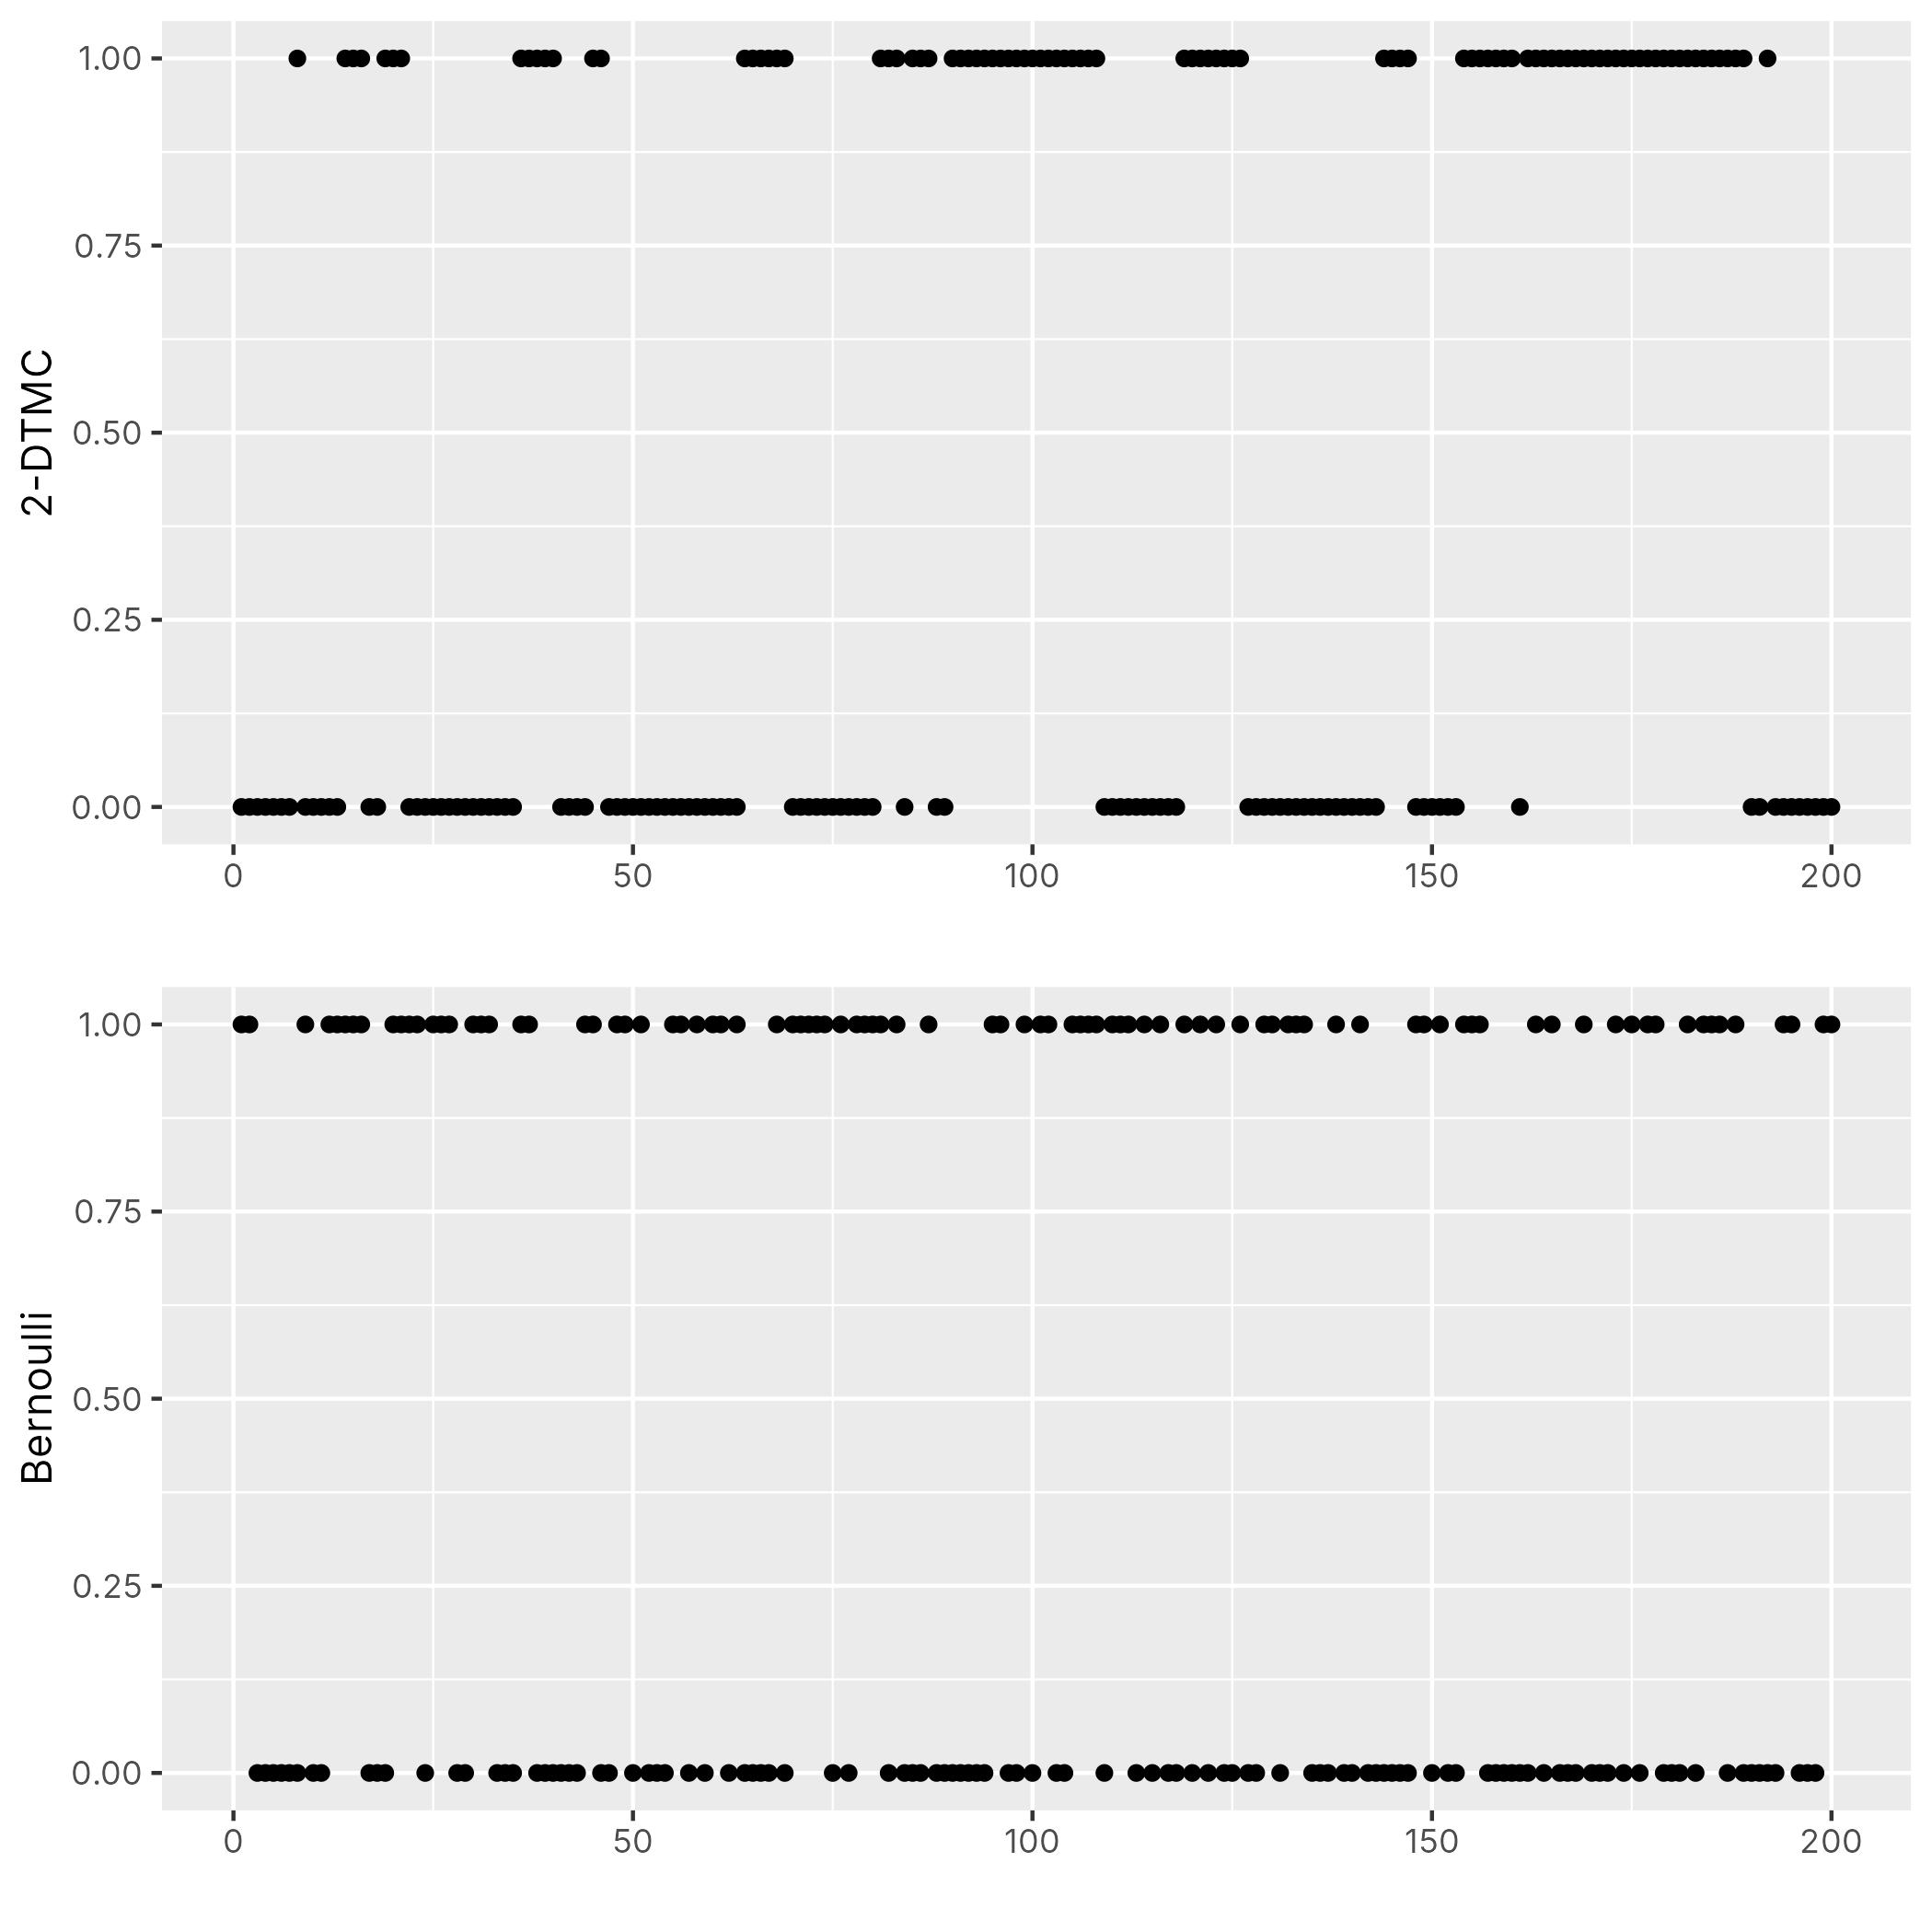
\includegraphics[width=\linewidth]{figuras/ex1_A.jpeg}\\
  {\small (a) $\alpha=0{,}9$, $\beta=0{,}1$}
\end{minipage}\hfill
\begin{minipage}{0.32\textwidth}\centering
  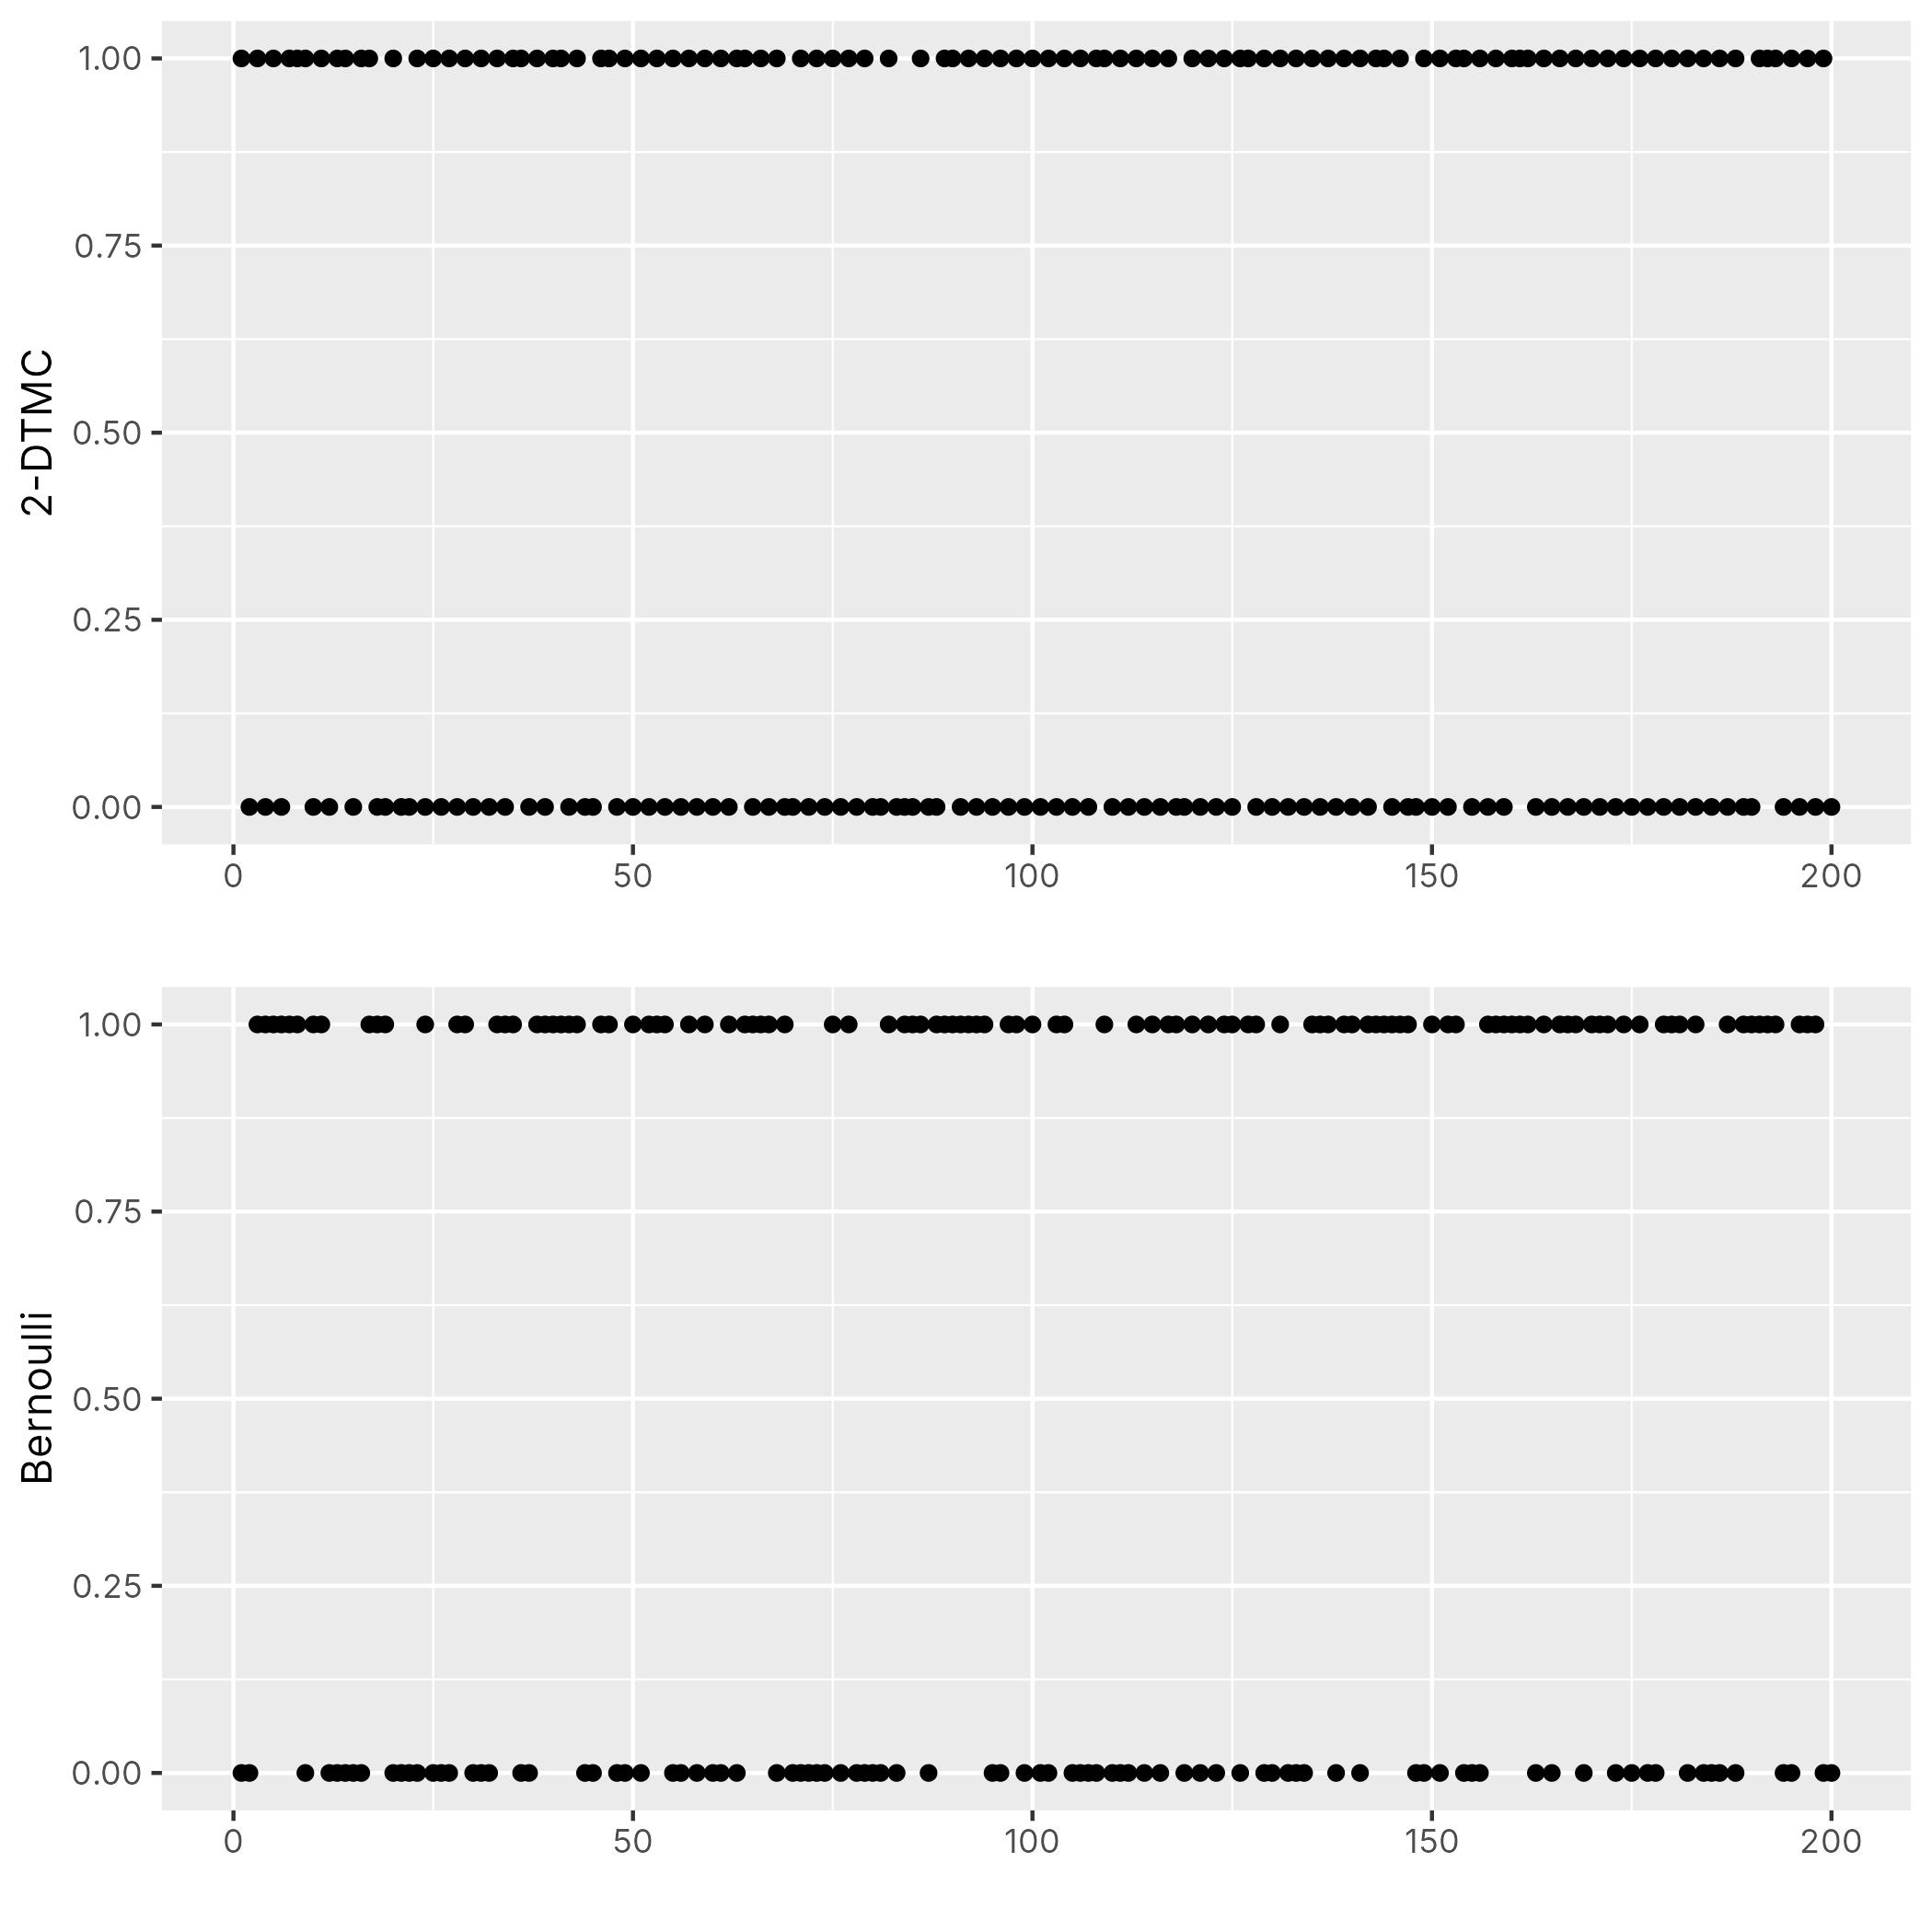
\includegraphics[width=\linewidth]{figuras/ex1_B.jpeg}\\
  {\small (b) $\alpha=0{,}1$, $\beta=0{,}9$}
\end{minipage}\hfill
\begin{minipage}{0.32\textwidth}\centering
  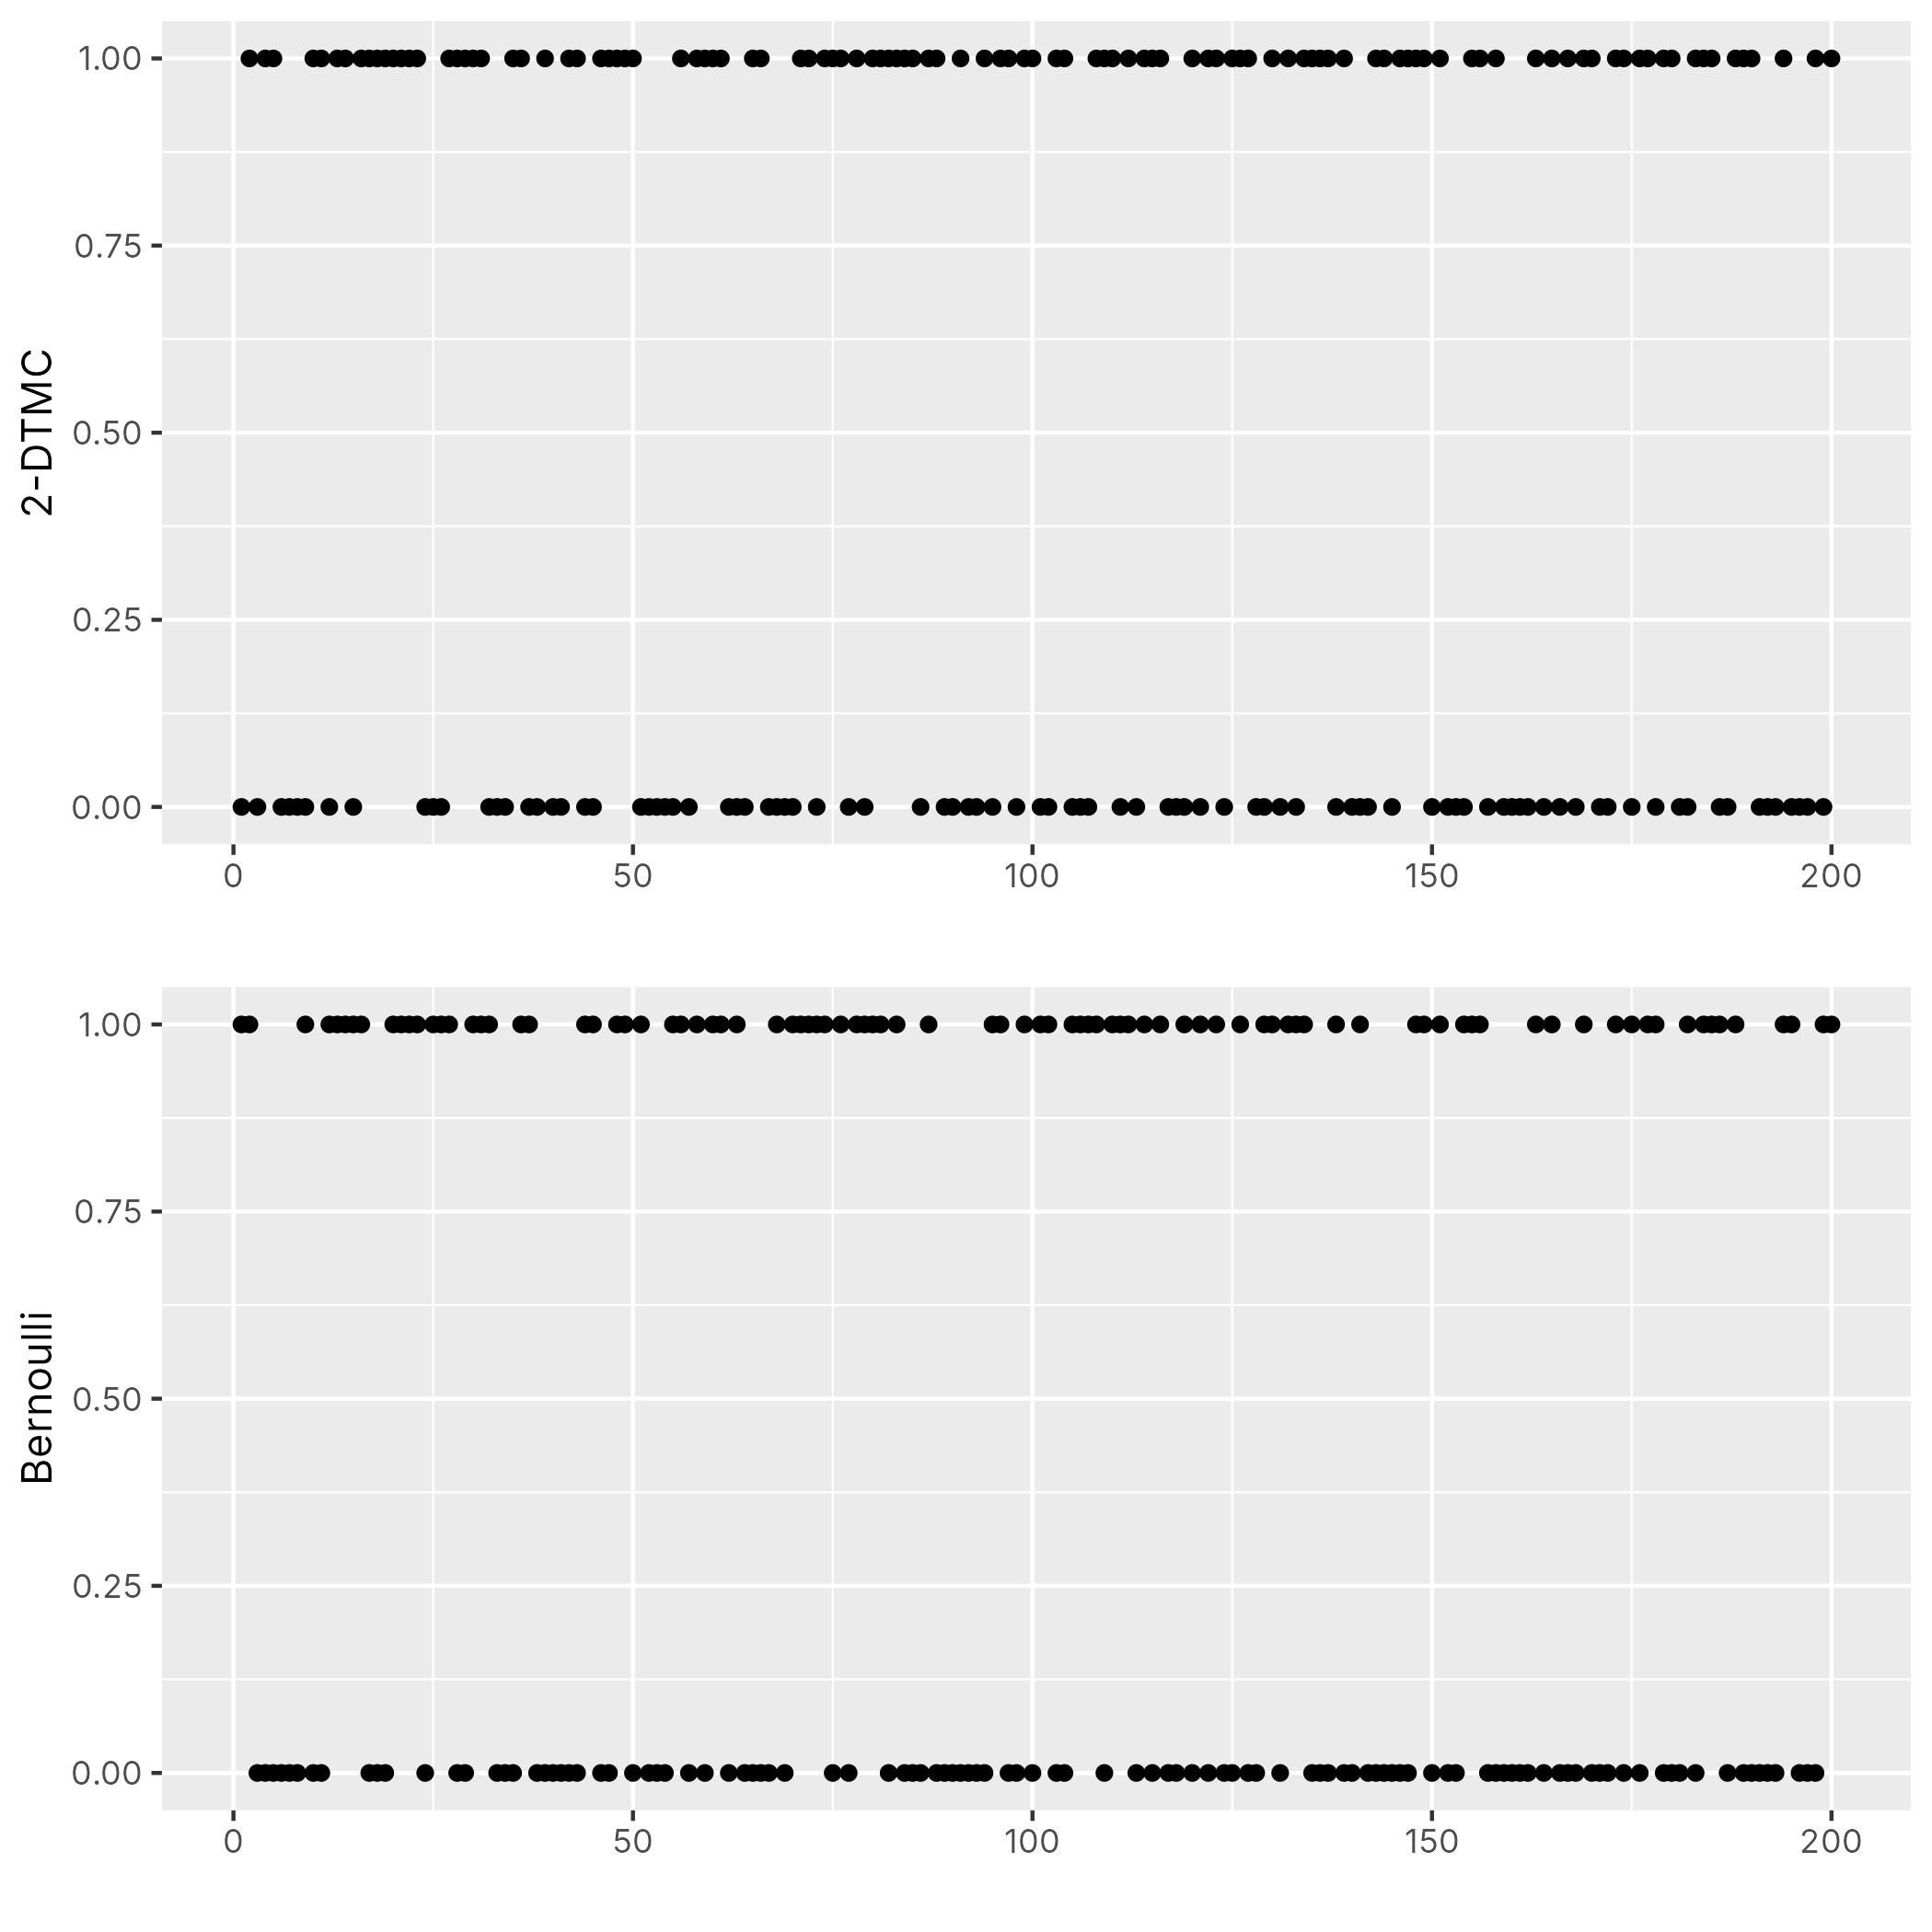
\includegraphics[width=\linewidth]{figuras/ex1_C.jpeg}\\
  {\small (c) $\alpha=0{,}5$, $\beta=0{,}5$}
\end{minipage}
\caption{Trajetórias de 200 \textit{slots} da 2-DTMC (em cima) e do processo de Bernoulli com a mesma média (em baixo).}
\label{fig:ex01}
\end{figure}

No caso A, a 2-DTMC permanece no mesmo estado com probabilidade 0,9 (Equação~\ref{eq:P}), o que produz longos períodos consecutivos de 0 e de 1 (rajadas). O processo de Bernoulli com a mesma média muda de estado com muito mais frequência e não apresenta rajadas. No caso B acontece o contrário: a 2-DTMC muda de estado com probabilidade 0,9 em cada \textit{slot} e alterna quase sempre entre 0 e 1, um padrão regular que o processo de Bernoulli também não reproduz. No caso C ($\alpha=\beta$), o estado seguinte não depende do estado atual e a 2-DTMC é equivalente ao processo de Bernoulli, como se confirma pelas trajetórias semelhantes da Figura~\ref{fig:ex01}(c).

Conclui-se que a 2-DTMC consegue modelar dependência entre \textit{slots} consecutivos, positiva (rajadas, por exemplo tráfego em rajada ou erros em rajada num canal) ou negativa (alternância). O processo de Bernoulli só modela \textit{slots} independentes: tem um único parâmetro, que fixa ao mesmo tempo a média e a duração dos períodos, enquanto a 2-DTMC tem dois parâmetros e permite escolher a duração dos períodos para a mesma média. O processo de Bernoulli é o caso particular $\alpha=\beta$ da 2-DTMC.

% ---------------------------------------------------------------
\subsection{Exercício 2: Estimação das probabilidades de transição}

O ficheiro \texttt{2dtmcdata.txt} contém \num{2000} dias consecutivos, em que o estado 0 representa um dia sem ataque e o estado 1 um dia com ataque. O \textit{script} converte o conjunto de dados num vetor ordenado e forma os \num{1999} pares de dias consecutivos $(x_t, x_{t+1})$. Para cada par de estados $(i,j)$ conta o número de transições $n_{ij}$ e estima a probabilidade de transição com a Equação~\ref{eq:estim}, ou seja, como a fração das transições que saem de $i$ e chegam a $j$. Os resultados encontram-se na Tabela~\ref{tab:ex02}.

\formula{\hat{p}_{ij} = \frac{n_{ij}}{\sum_{k} n_{ik}}, \qquad i,j \in \{0,1\}}{Estimador das probabilidades de transição.}{eq:estim}

\begin{table}[H]
\centering
\begin{tabular}{cccS[table-format=1.4]}
\toprule
Estado atual & Estado seguinte & {Contagem $n_{ij}$} & {Probabilidade $\hat{p}_{ij}$}\\
\midrule
0 & 0 & 623 & 0.5192\\
0 & 1 & 577 & 0.4808\\
1 & 0 & 577 & 0.7222\\
1 & 1 & 222 & 0.2778\\
\bottomrule
\end{tabular}
\caption{Contagens e probabilidades de transição estimadas da 2-DTMC.}
\label{tab:ex02}
\end{table}

A probabilidade de o servidor ser atacado num dia em que já foi atacado no dia anterior ($\hat{p}_{11}=0{,}278$) é inferior à de ser atacado após um dia sem ataque ($\hat{p}_{01}=0{,}481$). Os ataques tendem assim a não ocorrer em dias consecutivos. Como se viu no Exercício~1, um processo de Bernoulli não conseguiria representar este comportamento, porque assume dias independentes.

Como verificação, a probabilidade estacionária de ataque obtida com a Equação~\ref{eq:media} a partir das estimativas, $\pi_1=\hat{p}_{01}/(\hat{p}_{01}+\hat{p}_{10})=0{,}400$, coincide com a fração de dias atacados no conjunto de dados ($799/\num{2000}=0{,}3995$). A igualdade $n_{01}=n_{10}=577$ também é esperada: cada período de ataques começa com uma transição $0\to1$ e termina com uma transição $1\to0$, e a sequência começa e acaba no estado 0.

% ---------------------------------------------------------------
\subsection{Exercício 3: \textit{Throughput} do \textit{slotted} ALOHA com \texorpdfstring{$N$}{N} utilizadores}

\subsubsection*{a) \textit{Throughput} teórico}

A Figura~\ref{fig:aloha_theo} apresenta o \textit{throughput} teórico obtido com \texttt{aloha\_theo()}, através do \textit{script} \texttt{aloha\_plot.R}.

\begin{figure}[H]
\centering
\begin{minipage}{0.45\textwidth}\centering
  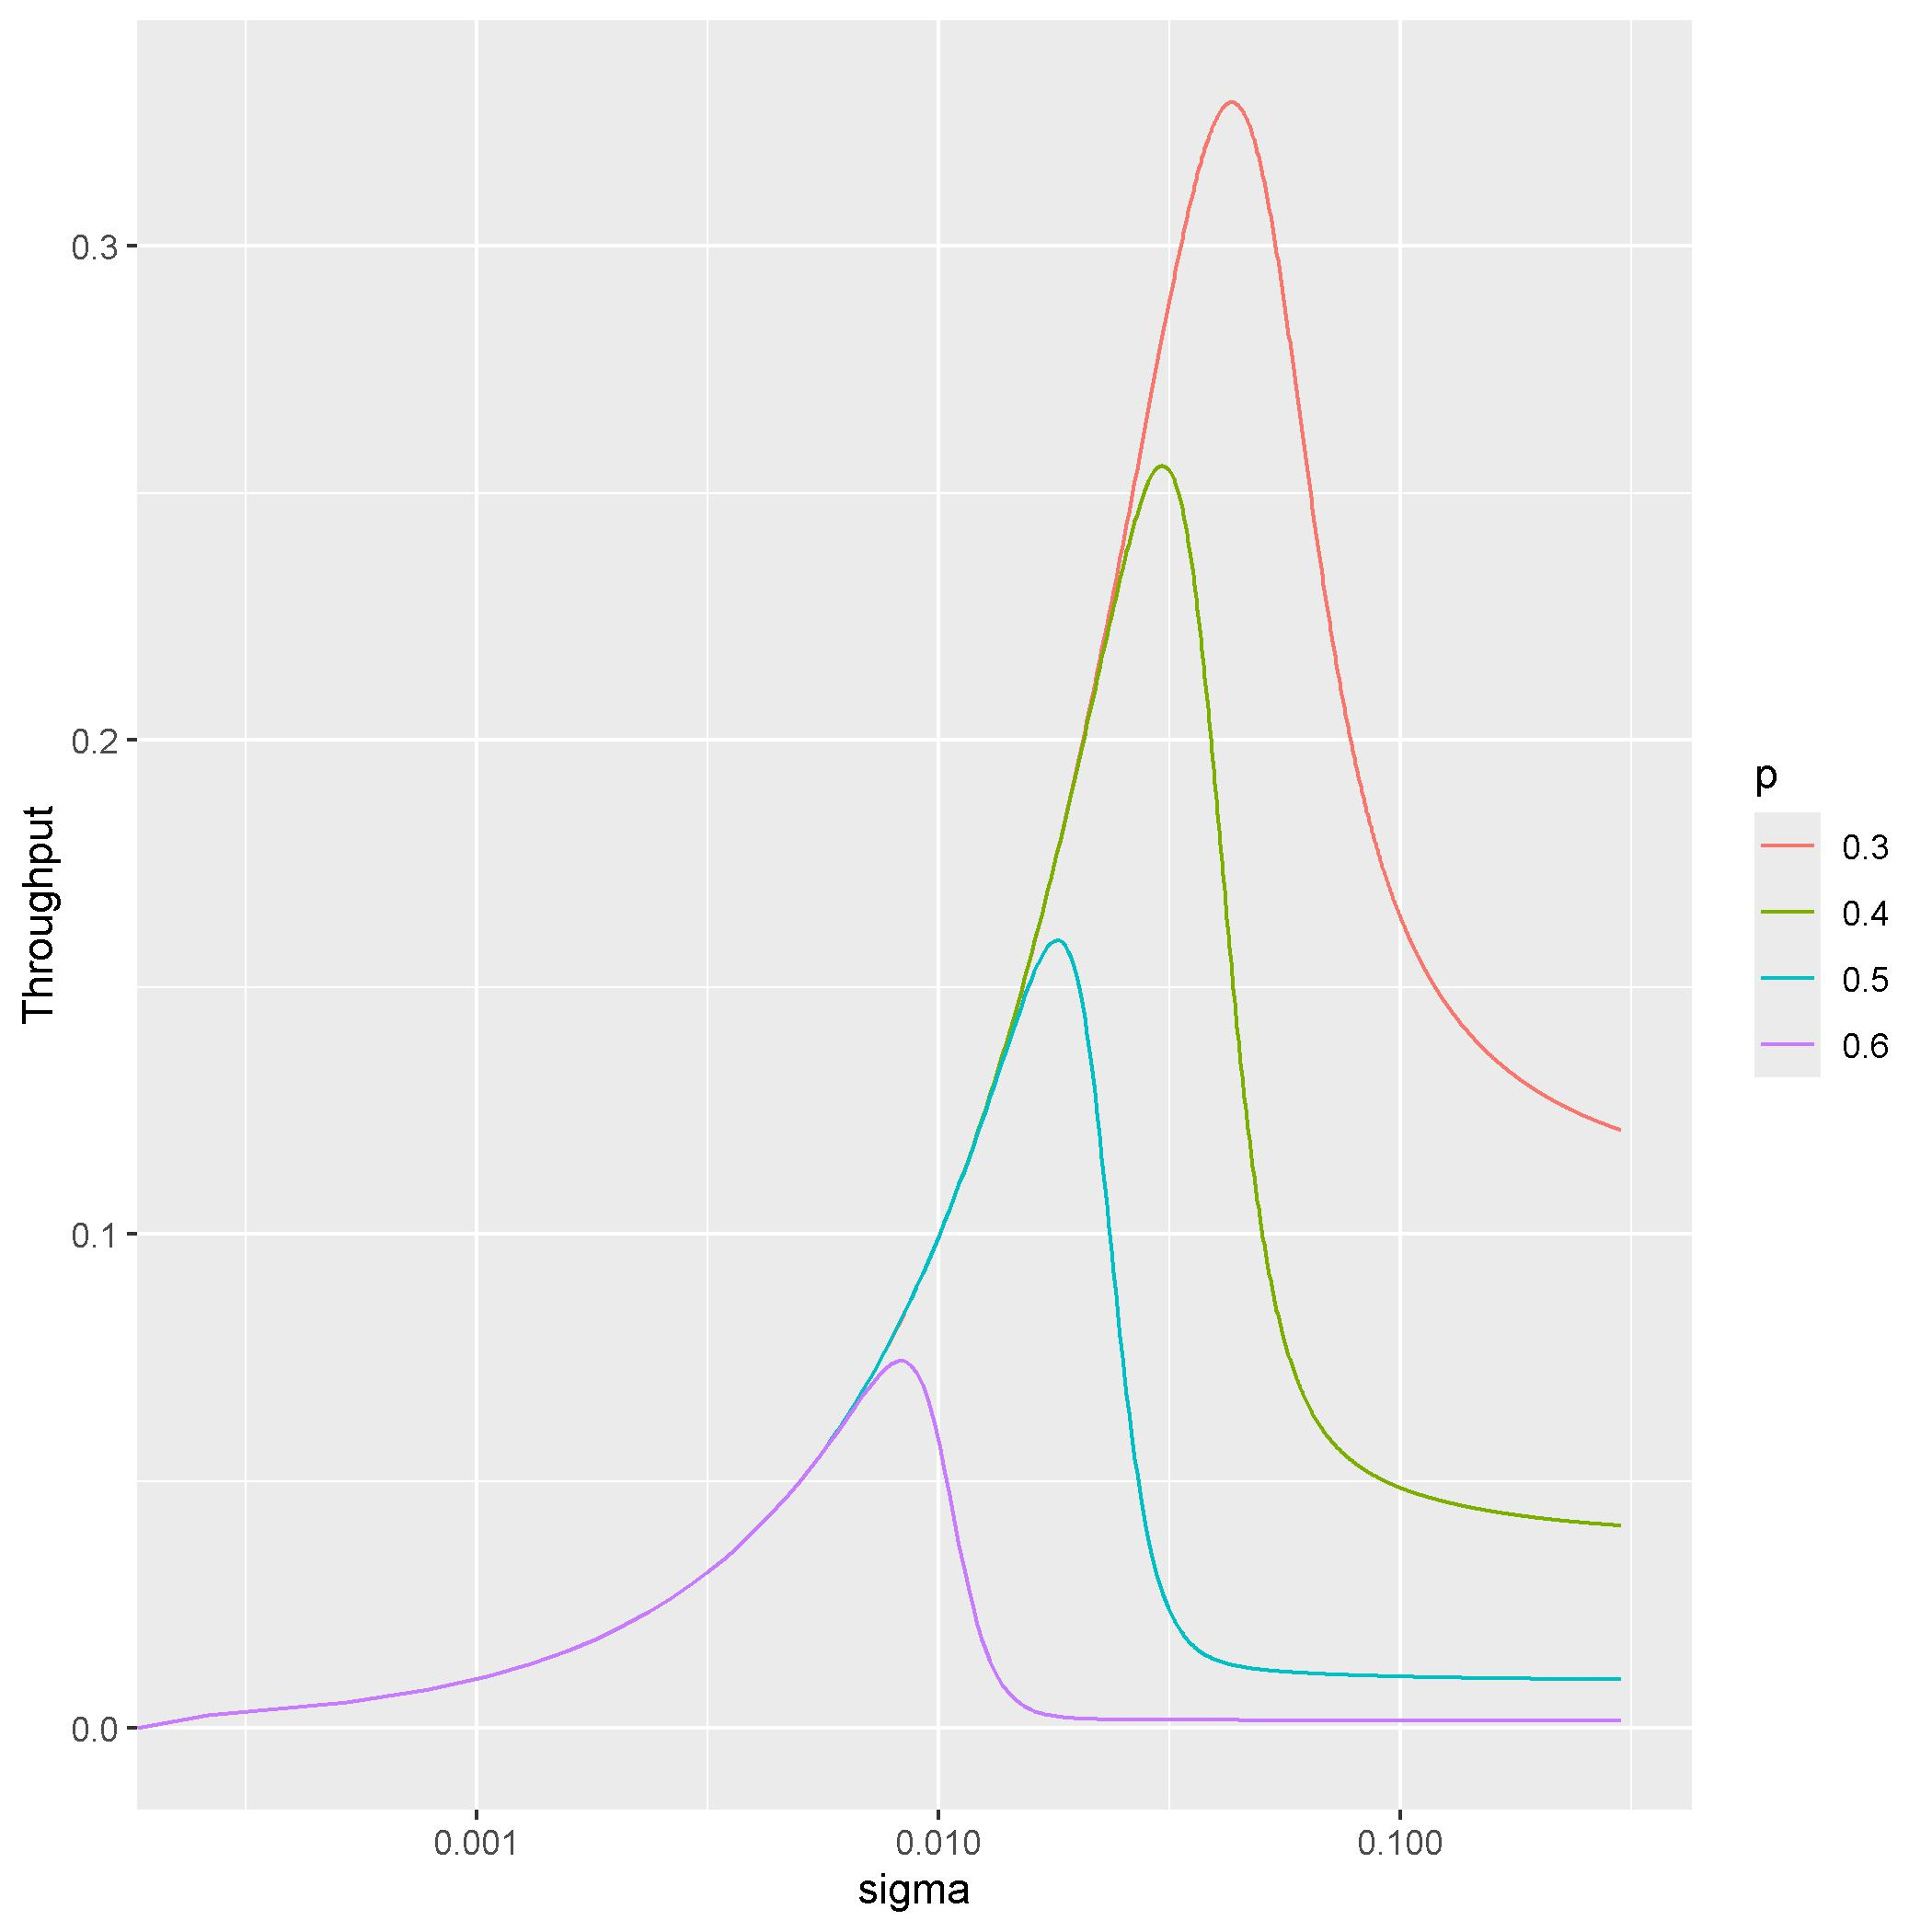
\includegraphics[width=\linewidth]{figuras/aloha10.jpeg}\\
  {\small (a) $N=10$}
\end{minipage}\hfill
\begin{minipage}{0.45\textwidth}\centering
  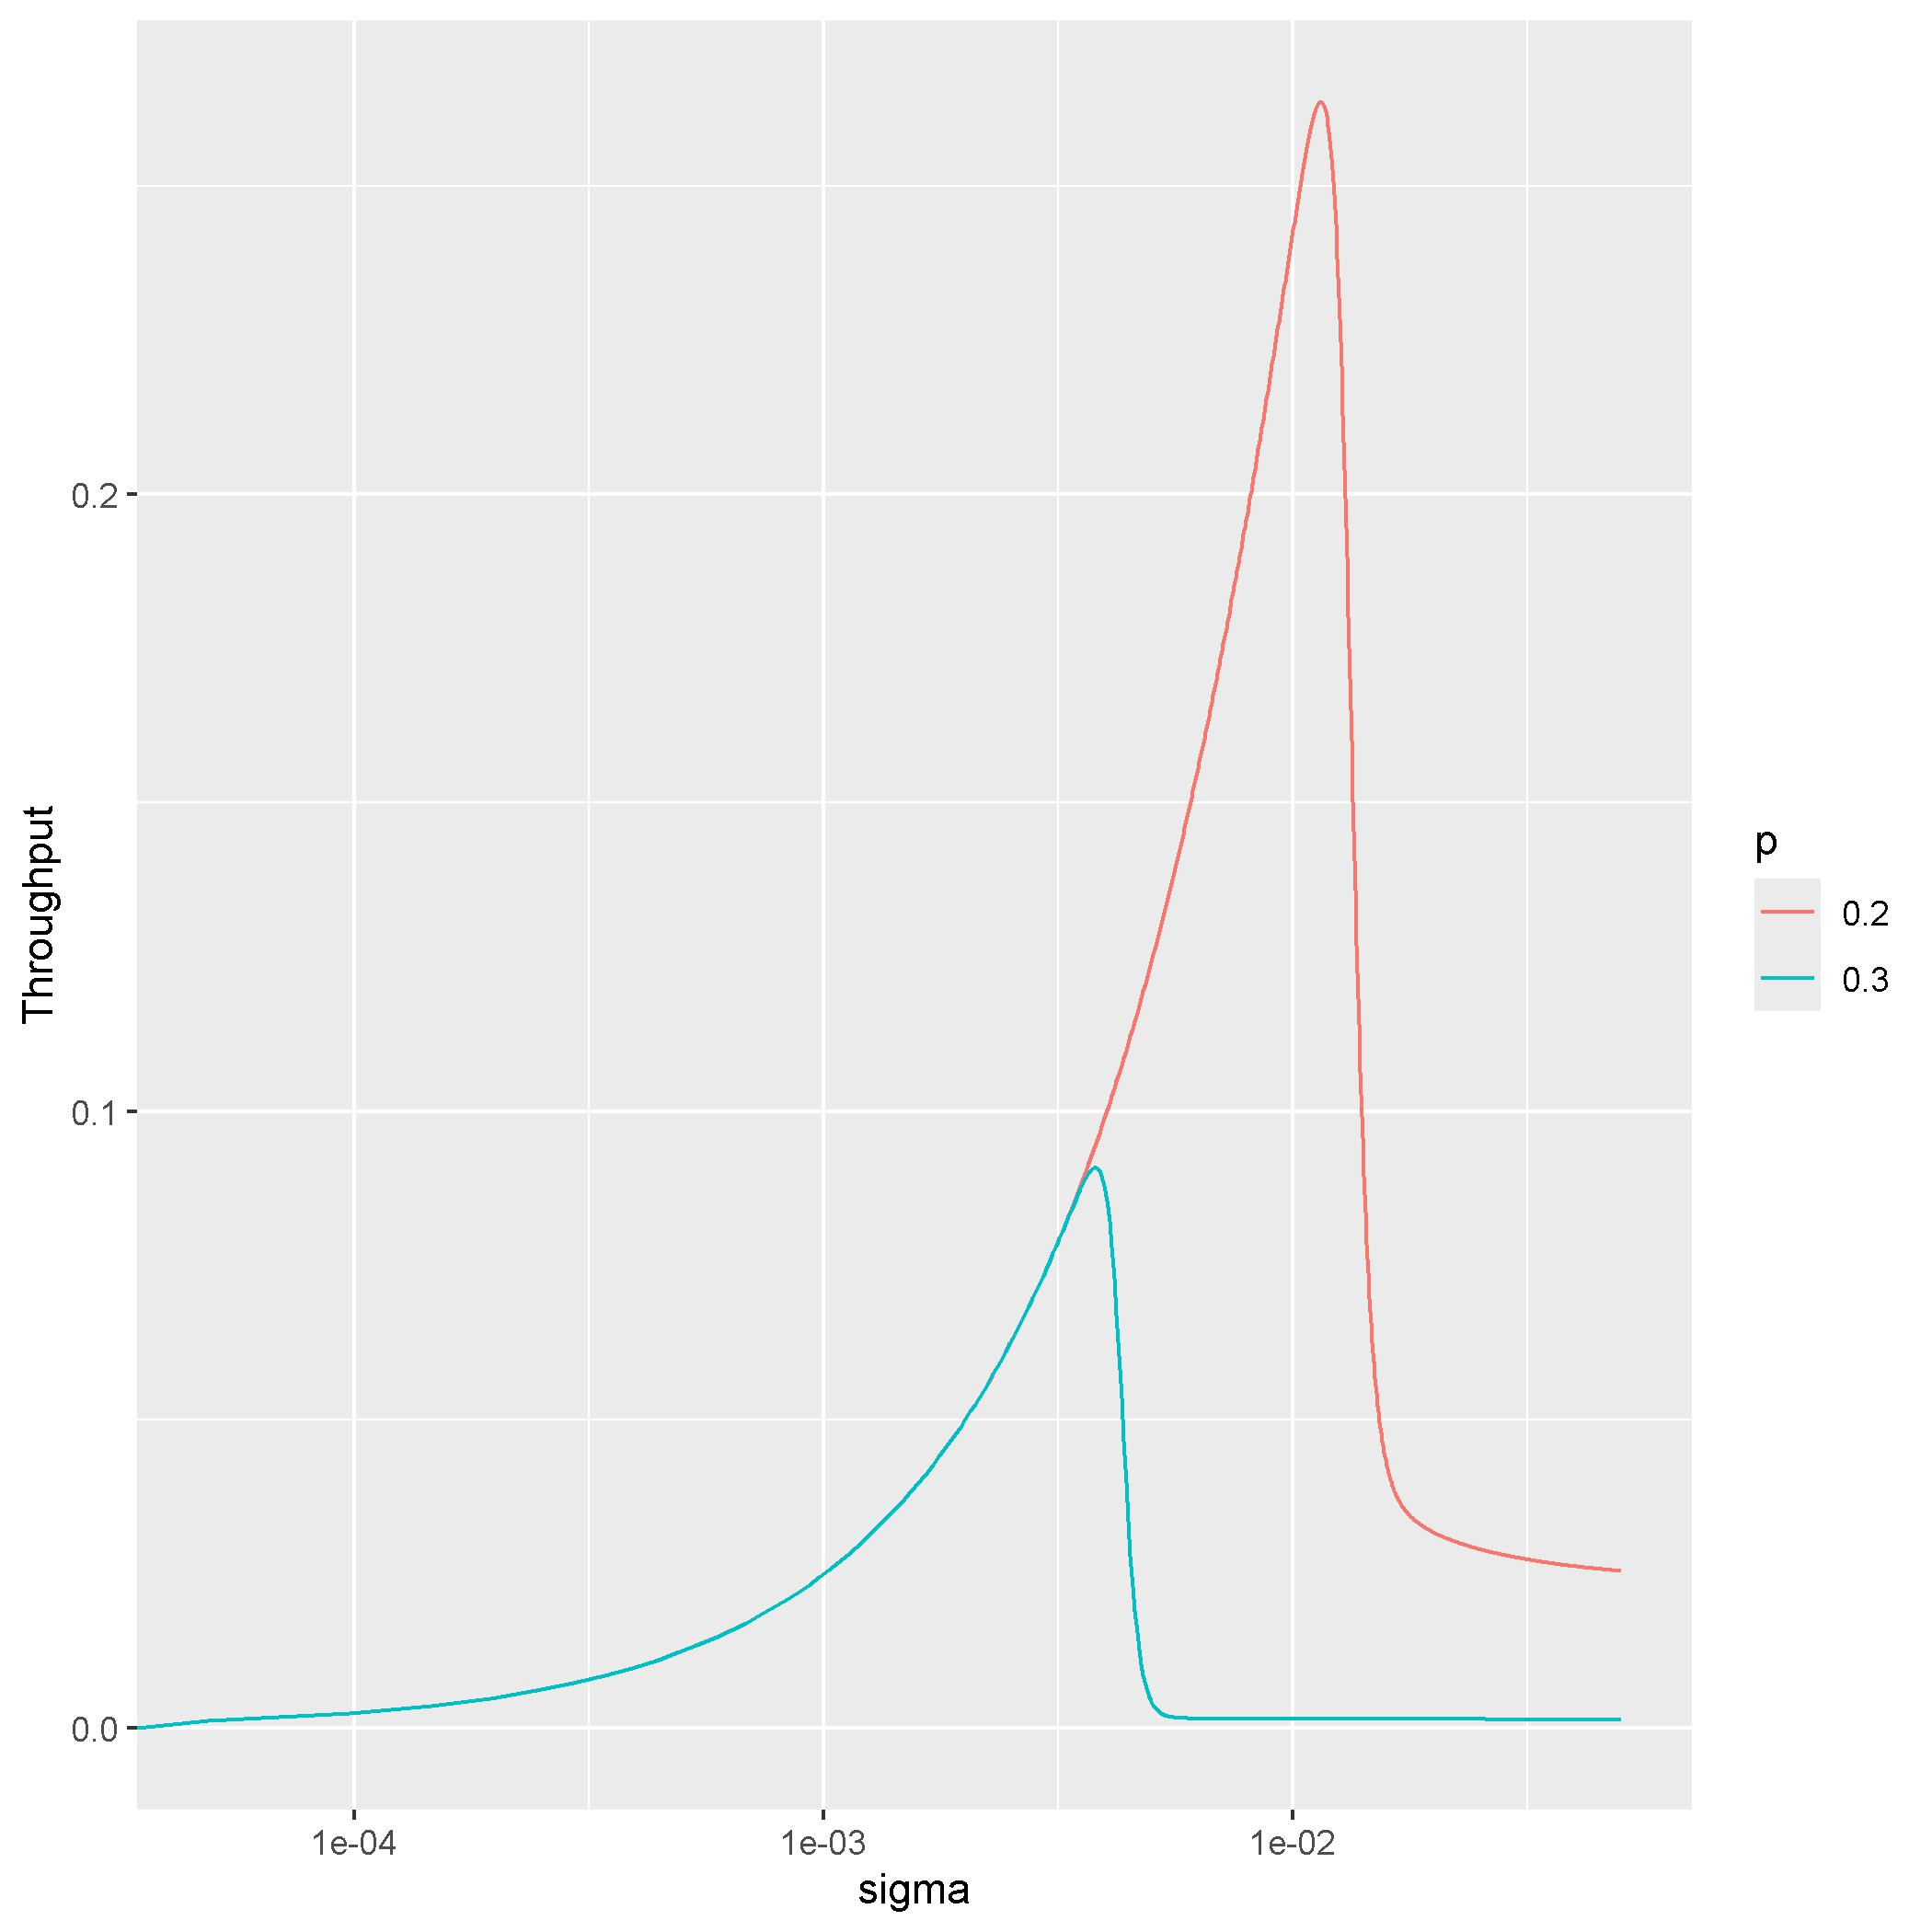
\includegraphics[width=\linewidth]{figuras/aloha25.jpeg}\\
  {\small (b) $N=25$}
\end{minipage}
\caption{\textit{Throughput} teórico do \textit{slotted} ALOHA em função de $\sigma$ (escala logarítmica), para vários valores de $p$.}
\label{fig:aloha_theo}
\end{figure}

\textbf{Efeito de $\sigma$:} para $\sigma$ baixo, quase não há colisões, quase nenhum utilizador está BACKLOGGED e o \textit{throughput} é aproximadamente igual à carga oferecida, $N\sigma$. Por isso as curvas de diferentes $p$ coincidem nesta zona. À medida que $\sigma$ aumenta, o \textit{throughput} cresce até um máximo e depois cai de forma abrupta: as colisões levam utilizadores para o estado BACKLOGGED, as suas retransmissões provocam novas colisões e o sistema entra num ciclo de realimentação positiva. Para $\sigma$ elevado, quase todos os utilizadores estão BACKLOGGED e o \textit{throughput} aproxima-se da probabilidade de sucesso com os $N$ utilizadores BACKLOGGED, $P_{suc}(N)=Np(1-p)^{N-1}$ (caso $i=N$ da probabilidade de sucesso condicionada do modelo), por exemplo cerca de 0,12 para $N=10$ e $p=0{,}3$, valor a que tende a curva respetiva.

\textbf{Efeito de $p$:} quanto menor $p$, maior o \textit{throughput} máximo e maior o valor de $\sigma$ a partir do qual o sistema colapsa. Para $N=10$, o máximo desce de cerca de 0,33 com $p=0{,}3$ para cerca de 0,07 com $p=0{,}6$. Quando há muitos utilizadores BACKLOGGED, um $p$ elevado faz com que vários retransmitam no mesmo \textit{slot} e colidam, pelo que reduzir $p$ diminui as colisões entre retransmissões. Em contrapartida, um $p$ menor aumenta o tempo que cada pacote espera até ser retransmitido.

\newpage

\textbf{Efeito de $N$:} para o mesmo $p=0{,}3$, passar de $N=10$ para $N=25$ reduz o \textit{throughput} máximo de cerca de 0,33 para cerca de 0,09, e o máximo passa a ocorrer num valor de $\sigma$ cerca de dez vezes menor. Com mais utilizadores, o mesmo $\sigma$ corresponde a uma carga total maior e há mais utilizadores que podem ficar BACKLOGGED e colidir. Para manter um \textit{throughput} elevado com mais utilizadores é necessário reduzir $p$: com $N=25$ e $p=0{,}2$, o máximo volta a cerca de 0,26.

\subsubsection*{b) Simulação por eventos discretos}

O simulador não modela o estado de cada utilizador. Como os utilizadores são idênticos, basta guardar o número $n$ de utilizadores no estado BACKLOGGED, que é o estado da cadeia de Markov usada em \texttt{aloha\_theo()}. Em cada \textit{slot}:
\begin{itemize}
  \item o número de transmissões de utilizadores THINKING é gerado como $A\sim\mathrm{Bin}(N-n,\sigma)$ e o de utilizadores BACKLOGGED como $B\sim\mathrm{Bin}(n,p)$;
  \item se $A+B=1$, há sucesso e conta-se um pacote transmitido; se o pacote pertencia a um utilizador BACKLOGGED, este volta a THINKING ($n\leftarrow n-1$);
  \item se $A+B\geq2$, há colisão e os $A$ utilizadores THINKING que transmitiram passam a BACKLOGGED ($n\leftarrow n+A$).
\end{itemize}
O \textit{throughput} é o número de sucessos a dividir pelo número de \textit{slots} simulados. Cada simulação começa com $n=0$ e corre \num{210000} \textit{slots}, dos quais os primeiros \num{10000} são descartados como período de aquecimento (\textit{warm-up}). Para cada conjunto de parâmetros foram realizadas $R=10$ simulações independentes. O intervalo de confiança a 95\% foi calculado com a Equação~\ref{eq:ic} e o erro relativo face ao valor teórico com a Equação~\ref{eq:erro}.

\formula{\bar{x}\pm t_{0{,}975;\,R-1}\,\frac{s}{\sqrt{R}}}{Intervalo de confiança a 95\% ($\bar{x}$: média e $s$: desvio padrão das $R$ simulações; $t$: quantil da distribuição \textit{t} de Student).}{eq:ic}

\formula{\varepsilon=\frac{\lvert \bar{x}-S_{\mathrm{teo}}\rvert}{S_{\mathrm{teo}}}\times100\%}{Erro relativo do \textit{throughput} simulado face ao teórico.}{eq:erro}

\begin{table}[H]
\centering
\begin{tabular}{S[table-format=2.0]S[table-format=1.2]S[table-format=1.2]cS[table-format=1.4]S[table-format=1.2]}
\toprule
{$N$} & {$\sigma$} & {$p$} & {Simulado} & {Teórico} & {Erro relativo (\%)}\\
\midrule
10 & 0.01 & 0.10 & $0{,}0986\pm0{,}0004$ & 0.0989 & 0.33\\
10 & 0.05 & 0.20 & $0{,}3677\pm0{,}0009$ & 0.3678 & 0.00\\
20 & 0.10 & 0.30 & $0{,}0071\pm0{,}0002$ & 0.0070 & 1.85\\
50 & 0.02 & 0.05 & $0{,}2540\pm0{,}0011$ & 0.2539 & 0.06\\
\bottomrule
\end{tabular}
\caption{\textit{Throughput} simulado (média $\pm$ semi-amplitude do IC a 95\%, 10 simulações) e teórico.}
\label{tab:ex03b}
\end{table}

Em todos os casos o valor teórico está dentro do intervalo de confiança da simulação, o que valida o simulador e o modelo teórico. O erro relativo é inferior a 0,4\%, exceto no terceiro conjunto (1,85\%). Este valor deve-se ao \textit{throughput} ser muito baixo (0,007): uma diferença absoluta pequena corresponde a um erro relativo maior, mas continua dentro do intervalo de confiança.

\newpage

Os quatro conjuntos de parâmetros levam a regimes de funcionamento distintos:
\begin{itemize}
  \item \textbf{Carga baixa} ($N=10$, $\sigma=0{,}01$): quase não há colisões e o \textit{throughput} (0,099) é praticamente igual à carga oferecida pelos utilizadores THINKING ($N\sigma=0{,}1$).
  \item \textbf{Próximo do ótimo} ($N=10$, $\sigma=0{,}05$, $p=0{,}2$): o \textit{throughput} (0,368) é próximo de $1/e$, o máximo do \textit{slotted} ALOHA com população infinita.
  \item \textbf{Colapso} ($N=20$, $\sigma=0{,}1$, $p=0{,}3$): a carga oferecida é demasiado elevada, praticamente todos os utilizadores ficam BACKLOGGED (segundo o modelo teórico, em média 19,9 em 20) e quase todos os \textit{slots} têm colisões, pelo que o \textit{throughput} cai para 0,007.
  \item \textbf{Muitos utilizadores, $p$ baixo} ($N=50$, $\sigma=0{,}02$, $p=0{,}05$): apesar de, segundo o modelo teórico, em média 37 dos 50 utilizadores estarem BACKLOGGED, a baixa probabilidade de retransmissão evita o colapso e mantém um \textit{throughput} de 0,254.
\end{itemize}

\subsubsection*{c) Comparação com CSMA e CSMA/CD}

No ALOHA as estações transmitem sem verificar se o canal está ocupado, pelo que qualquer transmissão pode colidir com outra que já esteja a decorrer. Um pacote só tem sucesso se nenhuma outra estação transmitir durante o seu período vulnerável, que no ALOHA puro corresponde a dois tempos de transmissão e no \textit{slotted} ALOHA a um só \textit{slot}. Por isso o \textit{throughput} máximo é baixo: cerca de 18\% no ALOHA puro e 37\% no \textit{slotted} ALOHA \cite{bertsekas1992}.

No CSMA (\textit{Carrier Sense Multiple Access}) cada estação escuta o canal antes de transmitir e só transmite se o encontrar livre. Assim, uma estação já não interrompe uma transmissão em curso e só há colisão quando duas estações começam a transmitir num intervalo inferior ao atraso de propagação, antes de uma detetar a outra. Quando o atraso de propagação é pequeno face ao tempo de transmissão de um pacote, as colisões tornam-se raras e o \textit{throughput} máximo pode ultrapassar 80\% \cite{kleinrock1975}.

No CSMA/CD (\textit{Collision Detection}) as estações continuam a escutar o canal enquanto transmitem e interrompem a transmissão assim que detetam uma colisão. Uma colisão passa a ocupar o canal apenas durante o tempo necessário para ser detetada, da ordem de duas vezes o atraso de propagação, e não durante a transmissão completa do pacote. Desperdiça-se ainda menos tempo e a eficiência pode aproximar-se de 100\% \cite{metcalfe1976}.

Assim, em termos de \textit{throughput}, ALOHA $<$ CSMA $<$ CSMA/CD. A vantagem do CSMA e do CSMA/CD diminui quando o atraso de propagação aumenta face ao tempo de transmissão, porque a informação obtida ao escutar o canal fica desatualizada.

Exemplos de tecnologias que usam cada protocolo:
\begin{itemize}
  \item \textbf{ALOHA:} a rede ALOHAnet da Universidade do Havai, onde o protocolo foi proposto \cite{abramson1970}, e o LoRaWAN, em que os dispositivos de classe A acedem ao canal com ALOHA puro \cite{lorawan}. A simplicidade do ALOHA é adequada a dispositivos IoT de baixo consumo e com pouco tráfego.
  \item \textbf{CSMA:} as redes Wi-Fi (IEEE 802.11) usam CSMA/CA, uma variante com prevenção de colisões e \textit{backoff} aleatório, porque num canal rádio uma estação não consegue detetar colisões enquanto transmite \cite{ieee80211}.
  \item \textbf{CSMA/CD:} a Ethernet clássica (IEEE 802.3) em modo \textit{half-duplex}, com barramento coaxial ou \textit{hubs} \cite{ieee8023}. A Ethernet comutada atual funciona em \textit{full-duplex}, cada ligação é ponto a ponto e não há colisões, pelo que o CSMA/CD deixou de ser usado.
\end{itemize}
\newpage

% ===============================================================
% B. Cadeias de Markov em tempo discreto e em tempo contínuo
% ===============================================================
\section{Cadeias de Markov em tempo discreto e em tempo contínuo}

% ---------------------------------------------------------------
\subsection{Exercício 4: Probabilidades limite de uma DTMC}

A DTMC de 3 estados do enunciado tem a matriz de transição da Equação~\ref{eq:P3}. As probabilidades limite foram obtidas de três formas.

\formula{P=\begin{bmatrix}0{,}6 & 0 & 0{,}4\\ 0{,}7 & 0{,}2 & 0{,}1\\ 0 & 0{,}2 & 0{,}8\end{bmatrix}}{Matriz de transição da DTMC de 3 estados.}{eq:P3}

\textbf{(i) Equações de balanço:} as equações de balanço $\boldsymbol{\pi}=\boldsymbol{\pi}P$, juntamente com a condição de normalização $\sum_j\pi_j=1$, foram resolvidas na forma matricial da Equação~\ref{eq:balanco}, em que $\mathbf{1}$ é um vetor linha de uns, $E$ uma matriz $3\times3$ de uns e $I$ a matriz identidade.

\formula{\boldsymbol{\pi}=\mathbf{1}\,(P+E-I)^{-1}}{Solução das equações de balanço da DTMC na forma matricial.}{eq:balanco}

\textbf{(ii) Multiplicação de matrizes:} pela equação de Chapman-Kolmogorov, a matriz de transição em $n$ passos é $P^n$ (Equação~\ref{eq:ck}), calculada com o operador \texttt{\%\^{}\%} do pacote \texttt{expm}. À medida que $n$ aumenta, as linhas de $P^n$ tornam-se iguais e cada linha converge para $\boldsymbol{\pi}$. Para $n=10$ as linhas já coincidem até à terceira casa decimal e para $n=20$ até à quarta, pelo que se usou $P^{20}$.

\formula{P^{(n)}=P^n,\qquad \pi_j=\lim_{n\to\infty}P^n_{ij}}{Equação de Chapman-Kolmogorov e probabilidades limite.}{eq:ck}

\textbf{(iii) Simulação:} a probabilidade limite $\pi_j$ corresponde também à fração de tempo que a cadeia passa no estado $j$. Por isso, gerou-se uma trajetória de \num{100000} transições, escolhendo em cada passo o estado seguinte com as probabilidades da linha do estado atual, e contou-se a fração de visitas a cada estado. Foram realizadas $R=10$ simulações independentes e calculado o intervalo de confiança a 95\% com a Equação~\ref{eq:ic}.

\begin{table}[H]
\centering
\begin{tabular}{cS[table-format=1.4]S[table-format=1.4]c}
\toprule
Estado & {(i) Equações de balanço} & {(ii) Multiplicação ($P^{20}$)} & {(iii) Simulação (IC 95\%)}\\
\midrule
0 & 0.2593 & 0.2593 & $0{,}2605\pm0{,}0016$\\
1 & 0.1481 & 0.1481 & $0{,}1479\pm0{,}0004$\\
2 & 0.5926 & 0.5926 & $0{,}5917\pm0{,}0016$\\
\bottomrule
\end{tabular}
\caption{Probabilidades limite da DTMC obtidas pelos três métodos.}
\label{tab:ex04}
\end{table}

Os três métodos dão resultados concordantes (Tabela~\ref{tab:ex04}). Os métodos (i) e (ii) são exatos e coincidem em todas as casas decimais apresentadas; os valores correspondem a $\boldsymbol{\pi}=(7/27,\,4/27,\,16/27)$. Na simulação, o valor teórico está dentro do intervalo de confiança em todos os estados. O método (i) é o mais direto, porque exige apenas a inversão de uma matriz. O método (ii) depende de se escolher um $n$ suficientemente grande, e a simulação dá apenas uma estimativa com erro estatístico, mas é a única abordagem aplicável quando o modelo é demasiado complexo para ser resolvido analiticamente.

% ---------------------------------------------------------------
\subsection{Exercício 5: Simulação de uma CTMC}

A CTMC de 3 estados do enunciado tem taxas de transição $\lambda_{12}=2$ e $\lambda_{21}=\lambda_{23}=\lambda_{31}=\lambda_{32}=1$. A taxa total de saída de cada estado é $\nu_i=\sum_j\lambda_{ij}$, que neste caso é igual a 2 nos três estados.

\textbf{Valores teóricos:} as probabilidades limite foram obtidas com a função \texttt{solve()} a partir das equações de balanço da Equação~\ref{eq:balctmc}, que igualam a taxa a que o processo sai de cada estado à taxa a que entra nele. Como as três equações são linearmente dependentes, usaram-se as equações dos estados 1 e 3 e a condição de normalização, o que dá $\boldsymbol{\pi}=(1/3,\,4/9,\,2/9)$.

\formula{\nu_j\pi_j=\sum_{i\neq j}\pi_i\lambda_{ij},\qquad \sum_j\pi_j=1}{Equações de balanço da CTMC.}{eq:balctmc}

\textbf{Simulação segundo a vista 1:} o processo permanece no estado $i$ durante um tempo exponencial de taxa $\nu_i$ e depois salta para o estado $j$ com a probabilidade da Equação~\ref{eq:psalto}, independentemente do tempo que passou em $i$.

\formula{P_{ij}=\frac{\lambda_{ij}}{\nu_i}}{Probabilidade de salto do estado $i$ para o estado $j$.}{eq:psalto}

\textbf{Simulação segundo a vista 2:} no estado $i$ gera-se, para cada transição possível, um tempo $T_j\sim\mathrm{Exp}(\lambda_{ij})$. O processo permanece em $i$ durante o menor destes tempos e transita para o estado correspondente a esse mínimo.

Nas duas vistas, a probabilidade limite de cada estado é estimada pela fração do tempo total que o processo passou nesse estado. Cada simulação dura \num{100000} unidades de tempo e começa no estado 1. Foram realizadas $R=10$ simulações independentes para cada vista e calculado o intervalo de confiança a 95\% com a Equação~\ref{eq:ic}.

\begin{table}[H]
\centering
\begin{tabular}{cS[table-format=1.4]cc}
\toprule
Estado & {Teórico} & {Vista 1 (IC 95\%)} & {Vista 2 (IC 95\%)}\\
\midrule
1 & 0.3333 & $0{,}3335\pm0{,}0007$ & $0{,}3330\pm0{,}0008$\\
2 & 0.4444 & $0{,}4441\pm0{,}0008$ & $0{,}4445\pm0{,}0006$\\
3 & 0.2222 & $0{,}2224\pm0{,}0011$ & $0{,}2225\pm0{,}0007$\\
\bottomrule
\end{tabular}
\caption{Probabilidades limite da CTMC: valores teóricos e estimativas por simulação segundo as duas vistas.}
\label{tab:ex05}
\end{table}

Em todos os estados, o valor teórico está dentro do intervalo de confiança das duas simulações (Tabela~\ref{tab:ex05}), e as duas vistas produzem estimativas com precisão semelhante. Isto confirma que as duas definições de CTMC são equivalentes: o mínimo de vários tempos exponenciais independentes de taxas $\lambda_{ij}$ é exponencial de taxa $\nu_i=\sum_j\lambda_{ij}$, e a probabilidade de o mínimo ser o tempo $T_j$ é $\lambda_{ij}/\nu_i=P_{ij}$.

\newpage

% ===============================================================
% C. Sistemas de filas de espera
% ===============================================================
\section{Sistemas de filas de espera}

% ---------------------------------------------------------------
\subsection{Exercício 6: Estabilidade do sistema M/M/1}

Foi usado o simulador M/M/1 fornecido, colocado dentro de uma função. A única alteração foi a forma de retirar clientes da fila: em vez de remover o primeiro elemento do vetor, usa-se um índice para o início da fila. Com $\rho\geq1$ a fila cresce sem limite e remover o primeiro elemento obrigava a copiar o vetor inteiro a cada partida, o que tornava as simulações longas demasiado lentas. A lógica do simulador não foi alterada.

A taxa de serviço foi fixada em $\mu=1$ e a taxa de chegada em $\lambda=\rho\mu$. Além de $\rho=1$ e $\rho=2$, simulou-se $\rho=0{,}5$ como referência de um sistema estável. Para cada valor de $\rho$ e de NumQueueCompleted ($N=10^3$, $10^4$ e $10^5$ clientes) foram realizadas $R=10$ simulações independentes e calculado o intervalo de confiança a 95\% com a Equação~\ref{eq:ic}. Para $\rho<1$, os resultados simulados foram comparados com o atraso médio na fila do M/M/1 (Equação~\ref{eq:mm1wq}). Para $\rho\geq1$ o atraso teórico é infinito, porque o sistema não tem regime estacionário e a fila cresce sem limite.

\formula{W_Q=\frac{\lambda}{\mu(\mu-\lambda)},\qquad \rho<1}{Atraso médio na fila do sistema M/M/1.}{eq:mm1wq}

\begin{table}[H]
\centering
\begin{tabular}{cS[table-format=6.0]cc}
\toprule
{$\rho$} & {$N$} & {Atraso médio na fila (IC 95\%)} & {Teórico}\\
\midrule
0,5 & 1000   & $1{,}07\pm0{,}14$ & 1,00\\
0,5 & 10000  & $1{,}01\pm0{,}03$ & 1,00\\
0,5 & 100000 & $1{,}01\pm0{,}02$ & 1,00\\
\midrule
1 & 1000   & $22{,}15\pm7{,}48$ & $+\infty$\\
1 & 10000  & $55{,}27\pm29{,}18$ & $+\infty$\\
1 & 100000 & $328{,}11\pm141{,}86$ & $+\infty$\\
\midrule
2 & 1000   & $257{,}47\pm13{,}70$ & $+\infty$\\
2 & 10000  & $2491{,}10\pm46{,}27$ & $+\infty$\\
2 & 100000 & $25043{,}18\pm158{,}43$ & $+\infty$\\
\bottomrule
\end{tabular}
\caption{Atraso médio na fila do M/M/1 em função do número de clientes simulados ($\mu=1$, 10 simulações por caso; $+\infty$: sem regime estacionário, o atraso cresce sem limite).}
\label{tab:ex06}
\end{table}

\begin{figure}[H]
\centering
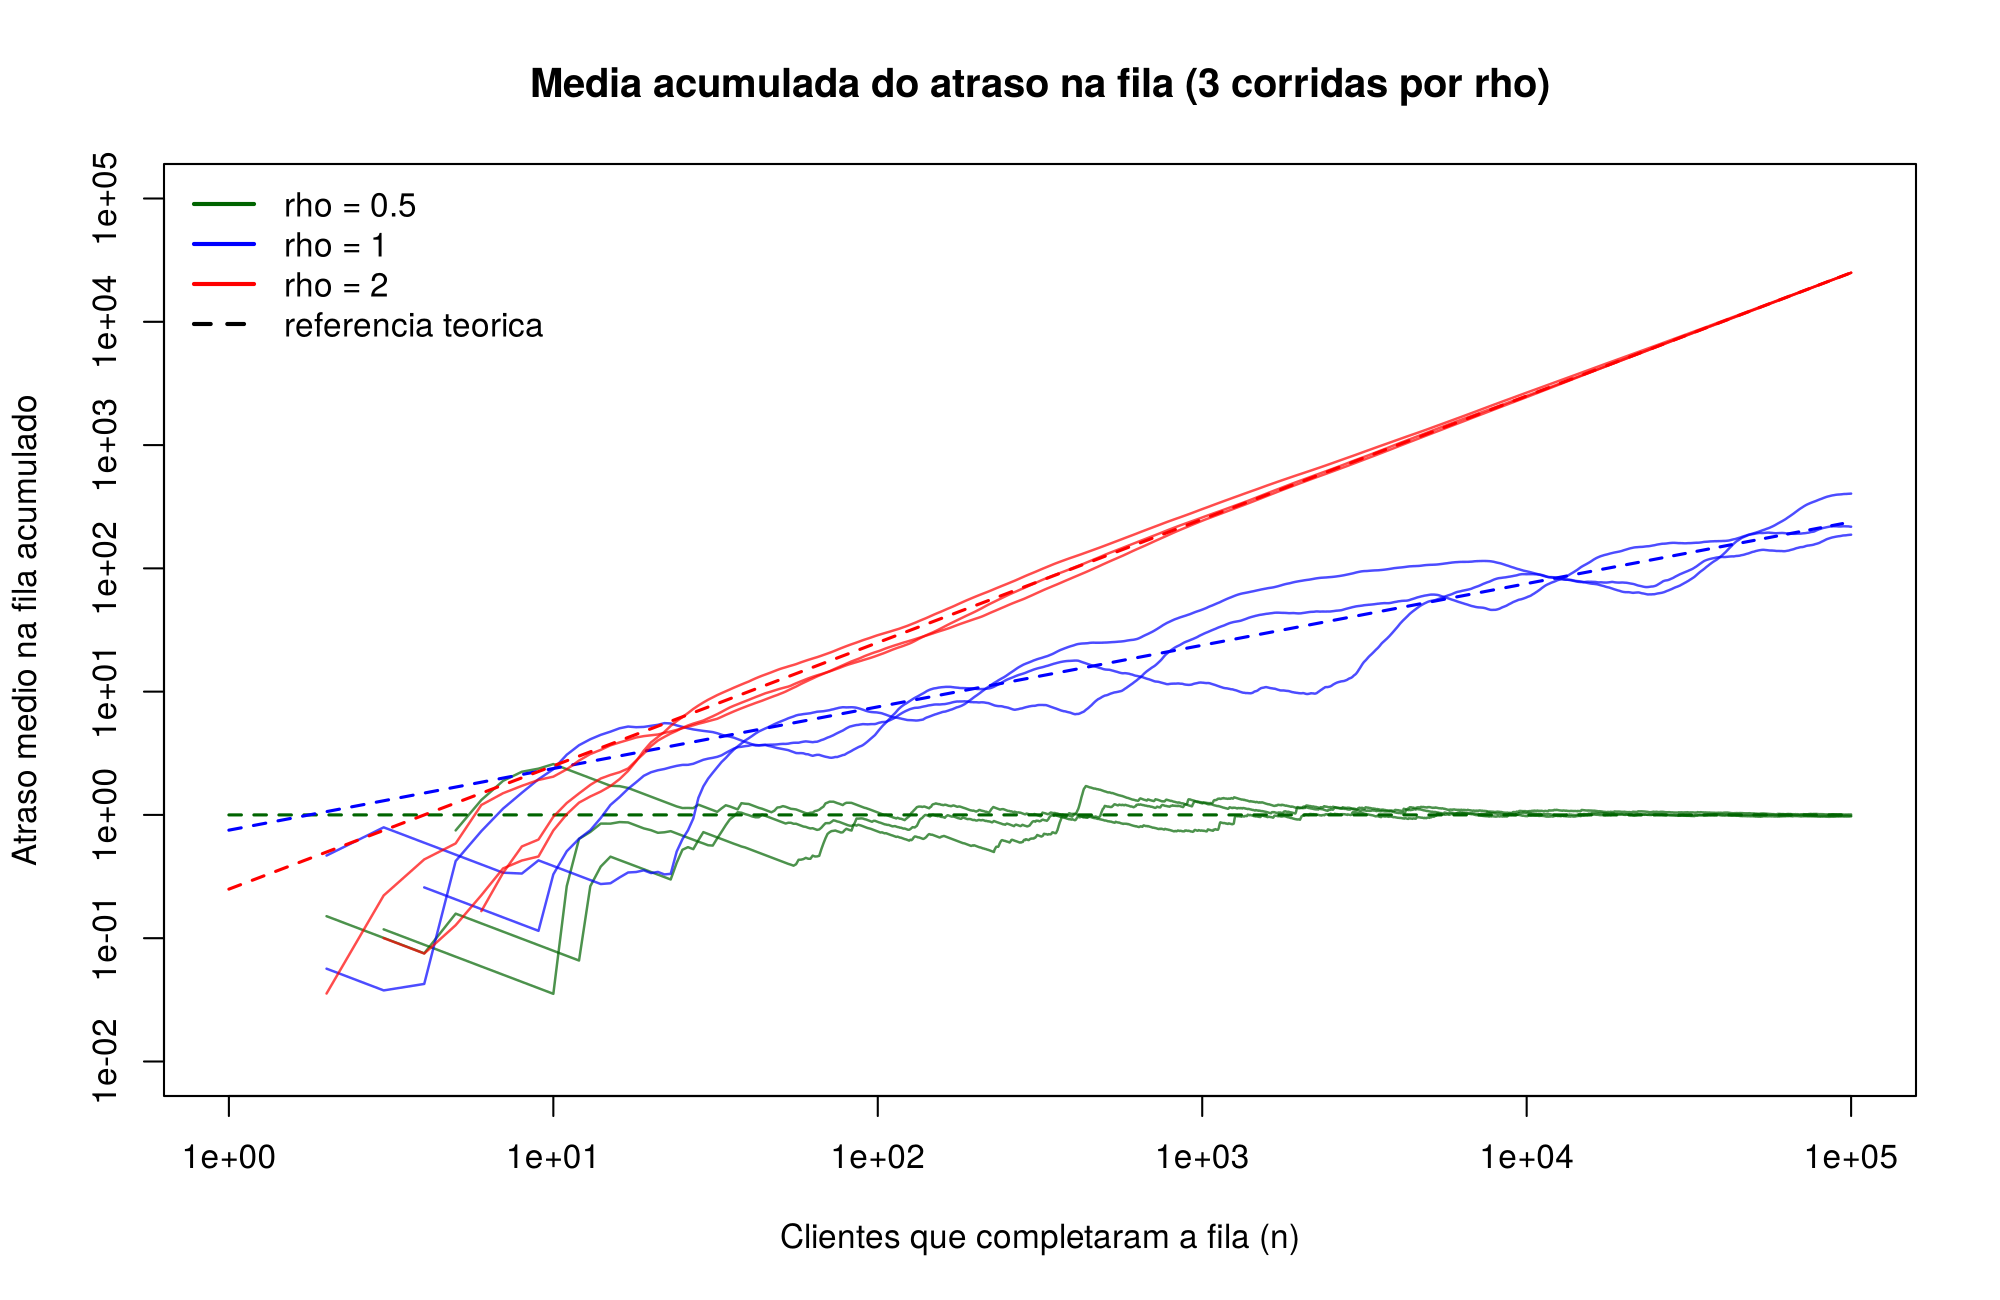
\includegraphics[width=0.75\textwidth]{figuras/ex6_media_acumulada.png}
\caption{Média acumulada do atraso na fila ao longo de três simulações por valor de $\rho$ (escalas logarítmicas); a tracejado, o valor teórico para $\rho=0{,}5$ (Equação~\ref{eq:mm1wq}).}
\label{fig:ex06}
\end{figure}

Com $\rho=0{,}5$ o atraso médio converge para o valor teórico de 1 e o intervalo de confiança diminui à medida que $N$ aumenta. Com $\rho=2$ chegam, em média, duas vezes mais clientes do que o servidor consegue atender, pelo que a fila cresce continuamente e cada cliente espera mais do que o anterior. O atraso médio cresce proporcionalmente a $N$: multiplica por 10 quando $N$ é multiplicado por 10. Com $\rho=1$ o atraso também cresce sem limite, mas mais lentamente e de forma irregular, com uma variabilidade muito elevada entre simulações: o intervalo de confiança chega a 50\% da média.

Conclui-se que, para $\rho=1$ e $\rho=2$, o sistema não é estável. A fila cresce sem limite, não existe regime estacionário e o atraso médio estimado depende apenas da duração da simulação: quanto mais longa a simulação, maior o atraso, pelo que o resultado não tem significado como medida de desempenho. A estabilidade do M/M/1 exige $\rho<1$, ou seja, que os clientes cheguem a uma taxa inferior à taxa a que o servidor os consegue atender.

% ---------------------------------------------------------------
\subsection{Exercício 7: Ligação ponto a ponto}

As simulações foram feitas com o simulador \texttt{ppl.R}. Nas alíneas a) e b), a ligação tem capacidade $C=100$~kb/s e serve dois fluxos iguais com tamanho médio de pacote $L=1000$ bits, pelo que $\mu=C/L=100$ pacotes/s. A carga total $\rho=\lambda/\mu$ é dividida igualmente pelos dois fluxos, cada um com taxa de chegada $\rho\mu/2$. Foram usados $\rho=0{,}5$ ($\lambda=25$ pacotes/s por fluxo) e $\rho=0{,}9$ ($\lambda=45$ pacotes/s por fluxo). O tempo de simulação segue a regra do \texttt{parameters.R}, $10000/\lambda$, ou seja 400~s e 222~s. Foram realizadas $R=10$ simulações independentes por caso e calculado o intervalo de confiança a 95\% com a Equação~\ref{eq:ic}. O atraso medido é o atraso no sistema (espera na fila e transmissão).

\subsubsection*{a) FIFO com pacotes de tamanho exponencial}

Com chegadas de Poisson e tamanhos exponenciais, a ligação é um sistema M/M/1, cujo atraso médio no sistema é dado pela Equação~\ref{eq:mm1w}, com $\lambda$ igual à soma das taxas dos dois fluxos.

\formula{W=\frac{1}{\mu-\lambda}}{Atraso médio no sistema M/M/1.}{eq:mm1w}

\begin{table}[H]
\centering
\begin{tabular}{ccS[table-format=3.0]cc}
\toprule
{$\rho$} & {$\lambda$ por fluxo (pacotes/s)} & {Teórico (ms)} & {Fluxo 1 (ms)} & {Fluxo 2 (ms)}\\
\midrule
0,5 & 25 & 20  & $19{,}82\pm0{,}40$ & $19{,}97\pm0{,}45$\\
0,9 & 45 & 100 & $100{,}02\pm9{,}74$ & $99{,}50\pm9{,}52$\\
\bottomrule
\end{tabular}
\caption{Atraso médio no sistema com FIFO e pacotes de tamanho exponencial: teórico e simulado (IC 95\%).}
\label{tab:ex07a}
\end{table}

Em todos os casos o valor teórico está dentro do intervalo de confiança (Tabela~\ref{tab:ex07a}). Os dois fluxos têm o mesmo atraso, porque com FIFO os pacotes são servidos por ordem de chegada, independentemente do fluxo. Quando a carga passa de 0,5 para 0,9, o atraso aumenta 5 vezes: o atraso do M/M/1 cresce com $1/(1-\rho)$ e torna-se muito sensível à carga quando esta se aproxima de 1. A precisão da simulação também diminui, com um intervalo de confiança de cerca de 10\% da média para $\rho=0{,}9$.

\subsubsection*{b) FIFO com pacotes de tamanho fixo}

Com pacotes de tamanho fixo, o tempo de serviço é constante e a ligação é um sistema M/D/1. O atraso médio no sistema obtém-se da fórmula de Pollaczek-Khinchine (Equação~\ref{eq:pk}), com $E[S]=1/\mu$ e $E[S^2]=1/\mu^2$.

\formula{W=\frac{\lambda E[S^2]}{2(1-\rho)}+E[S]=\frac{\rho}{2\mu(1-\rho)}+\frac{1}{\mu}}{Atraso médio no sistema M/G/1 (Pollaczek-Khinchine) e caso particular M/D/1.}{eq:pk}

\begin{table}[H]
\centering
\begin{tabular}{ccS[table-format=2.0]cc}
\toprule
{$\rho$} & {$\lambda$ por fluxo (pacotes/s)} & {Teórico (ms)} & {Fluxo 1 (ms)} & {Fluxo 2 (ms)}\\
\midrule
0,5 & 25 & 15 & $14{,}90\pm0{,}09$ & $14{,}97\pm0{,}07$\\
0,9 & 45 & 55 & $55{,}93\pm2{,}56$ & $56{,}11\pm2{,}59$\\
\bottomrule
\end{tabular}
\caption{Atraso médio no sistema com FIFO e pacotes de tamanho fixo: teórico e simulado (IC 95\%).}
\label{tab:ex07b}
\end{table}

A simulação concorda com a teoria (Tabela~\ref{tab:ex07b}). A única exceção é o fluxo 1 com $\rho=0{,}5$, cujo intervalo fica ligeiramente abaixo de 15~ms (até 14,98~ms). Com intervalos a 95\%, é esperado que cerca de 1 em cada 20 não contenha o valor teórico. Além disso, cada simulação começa com o sistema vazio, o que tende a subestimar ligeiramente o atraso.

Comparando com a alínea a), os pacotes de tamanho fixo têm um atraso bastante menor: 15~ms em vez de 20~ms com $\rho=0{,}5$, e 55~ms em vez de 100~ms com $\rho=0{,}9$. O tempo de transmissão é o mesmo nos dois casos (10~ms), mas o tempo de espera na fila do M/D/1 é metade do do M/M/1, porque $E[S^2]$ passa de $2/\mu^2$ para $1/\mu^2$. A diferença absoluta cresce com a carga. Os intervalos de confiança também são 4 a 7 vezes mais estreitos, porque há menos variabilidade. Conclui-se que, para a mesma carga, o desempenho de um sistema de filas não depende apenas do tempo médio de serviço mas também da sua variabilidade: quanto maior a variância do tempo de serviço, maior o atraso.

\subsubsection*{c) Prioridade estrita com pacotes de tamanho fixo}

A ligação ($C=100$~kb/s) serve dois fluxos com pacotes de tamanho fixo $L=1000$ bits ($\mu=100$ pacotes/s): o fluxo 1, de prioridade alta, com $\lambda_1=10$ pacotes/s ($\rho_1=0{,}1$), e o fluxo 2, de prioridade baixa, com $\lambda_2=85$ pacotes/s, o que dá uma carga total $\rho=0{,}95$. O tempo de simulação é $10000/\lambda_1=1000$~s e foram realizadas $R=10$ simulações independentes. O escalonamento é não preemptivo: um pacote de prioridade baixa em transmissão não é interrompido. Os valores teóricos foram obtidos com a Equação~\ref{eq:prio} (M/D/1 com prioridades estritas), somando o tempo de transmissão $1/\mu$ ao atraso na fila.

\formula{W_k=\frac{\rho/(2\mu)}{\left(1-\sum_{i=1}^{k}\rho_i\right)\left(1-\sum_{i=1}^{k-1}\rho_i\right)}+\frac{1}{\mu}}{Atraso médio no sistema da classe $k$ num M/D/1 com prioridades estritas não preemptivas.}{eq:prio}

\begin{table}[H]
\centering
\begin{tabular}{lS[table-format=3.2]c}
\toprule
 & {Teórico} & {Simulado (IC 95\%)}\\
\midrule
Fluxo 1, prioridade alta (ms) & 15.28 & $15{,}29\pm0{,}03$\\
Fluxo 2, prioridade baixa (ms) & 115.56 & $113{,}96\pm7{,}50$\\
Razão $W_2/W_1$ & 7.56 & $7{,}46\pm0{,}50$\\
\bottomrule
\end{tabular}
\caption{Atraso médio no sistema com prioridade estrita ($\lambda_1=10$, $\lambda_2=85$ pacotes/s, $\rho=0{,}95$): teórico e simulado (IC 95\%).}
\label{tab:ex07c}
\end{table}

Os valores teóricos estão dentro dos intervalos de confiança (Tabela~\ref{tab:ex07c}) e o atraso do fluxo de prioridade alta é cerca de 7,5 vezes menor do que o do fluxo de prioridade baixa, acima do mínimo de 4 pedido. O valor de $\lambda_2$ foi escolhido para que a razão teórica ficasse bem acima de 4. Com $\lambda_2=80$ ($\rho=0{,}9$) a razão teórica é exatamente 4 e a simulada ficou ligeiramente abaixo ($3{,}97\pm0{,}07$).

O fluxo de prioridade alta quase não é afetado pela carga do outro fluxo: só espera pelos pacotes do próprio fluxo, que são poucos, e pela conclusão do pacote que está a ser transmitido. Já o fluxo de prioridade baixa espera por todo o tráfego prioritário e suporta quase toda a carga do sistema. A prioridade não reduz o atraso médio global, apenas o redistribui: a média dos dois atrasos ponderada pelas taxas de chegada, $(10\times15{,}28+85\times115{,}56)/95=105$~ms, é igual ao atraso do M/D/1 com FIFO para $\rho=0{,}95$ (Equação~\ref{eq:pk}). A precisão da simulação é muito diferente nos dois fluxos (0,2\% e 6,6\% de semi-amplitude relativa), porque o fluxo de prioridade baixa funciona próximo da saturação.


\newpage

% ===============================================================
% D. Workloads
% ===============================================================
\section{\textit{Workloads}}

% ---------------------------------------------------------------
\subsection{Exercício 8: Impacto da variabilidade do tamanho dos trabalhos}

Foram comparados três sistemas com a mesma carga $\rho=0{,}5$ e o mesmo tempo médio de serviço $E[S]=2$ ($\mu=0{,}5$ e $\lambda=0{,}25$): um M/M/1 e dois M/G/1 com distribuição de serviço bimodal (\textit{mice-elephants}). No primeiro, Bimodal-1, 90\% dos trabalhos têm tamanho 1 (ratos) e 10\% têm tamanho 11 (elefantes); no segundo, Bimodal-2, 99\% têm tamanho 1 e 1\% tem tamanho 101. A variabilidade do tamanho dos trabalhos é medida pelo coeficiente de variação quadrático (Equação~\ref{eq:scv}), e o atraso médio na fila teórico foi obtido com a fórmula de Pollaczek-Khinchine (Equação~\ref{eq:pk}, sem a parcela $E[S]$).

\formula{E[S]=s_1p_1+s_2p_2,\qquad E[S^2]=s_1^2p_1+s_2^2p_2,\qquad C^2=\frac{E[S^2]}{E[S]^2}-1}{Momentos do tempo de serviço bimodal e coeficiente de variação quadrático.}{eq:scv}

As simulações usaram o \textit{script} \texttt{mg1\_bimodal.R}, em que cada simulação termina ao fim de \num{10000} clientes (StoppingCondition), alterando apenas os parâmetros $s_1$, $p_1$, $s_2$ e $p_2$ de cada sistema.

\subsubsection*{a) Atraso médio na fila}

Para cada sistema foram realizadas $R=20$ simulações independentes e calculado o intervalo de confiança a 95\% com a Equação~\ref{eq:ic}.

\begin{table}[H]
\centering
\begin{tabular}{lS[table-format=2.2]S[table-format=2.2]c}
\toprule
Sistema & {$C^2$} & {Teórico} & {Simulado (IC 95\%)}\\
\midrule
M/M/1 & 1.00 & 2.00 & $2{,}05\pm0{,}06$\\
M/Bimodal-1/1 & 2.25 & 3.25 & $3{,}19\pm0{,}06$\\
M/Bimodal-2/1 & 24.75 & 25.75 & $25{,}42\pm2{,}58$\\
\bottomrule
\end{tabular}
\caption{Atraso médio na fila do M/M/1 e dos dois M/G/1 bimodais ($\rho=0{,}5$, $E[S]=2$, 20 simulações por sistema).}
\label{tab:ex08a}
\end{table}

Os valores teóricos estão dentro dos intervalos de confiança e coincidem com os do slide de \textit{workloads} sobre o impacto da variabilidade (Tabela~\ref{tab:ex08a}). Embora a carga e o tempo médio de serviço sejam iguais nos três sistemas, o atraso médio na fila cresce com $C^2$: é 1,6 vezes maior no Bimodal-1 e cerca de 13 vezes maior no Bimodal-2 do que no M/M/1. Isto acontece porque o atraso depende de $E[S^2]$ e não só de $E[S]$. Os elefantes são raros mas ocupam o servidor durante muito tempo (101 unidades no Bimodal-2), e os muitos ratos que chegam entretanto ficam todos à espera. Conclui-se que a variabilidade da carga de trabalho degrada fortemente o desempenho, mesmo quando a carga média se mantém.

\subsubsection*{b) Variância das estimativas}

Para cada sistema foram obtidas 100 estimativas independentes do atraso médio na fila (100 simulações de \num{10000} clientes) e calculada a sua variância amostral.

\begin{table}[H]
\centering
\begin{tabular}{lS[table-format=2.2]S[table-format=2.2]S[table-format=2.4]S[table-format=2.4]S[table-format=4.1]}
\toprule
Sistema & {$C^2$} & {Média} & {Variância} & {Desvio padrão} & {Variância / variância M/M/1}\\
\midrule
M/M/1 & 1.00 & 2.01 & 0.0137 & 0.1170 & 1.0\\
M/Bimodal-1/1 & 2.25 & 3.23 & 0.0398 & 0.1994 & 2.9\\
M/Bimodal-2/1 & 24.75 & 25.75 & 23.8677 & 4.8855 & 1742.9\\
\bottomrule
\end{tabular}
\caption{Variância amostral de 100 estimativas do atraso médio na fila (\num{10000} clientes por simulação).}
\label{tab:ex08b}
\end{table}

A variância das estimativas aumenta muito com a variabilidade do tamanho dos trabalhos (Tabela~\ref{tab:ex08b}): é cerca de 3 vezes maior no Bimodal-1 e cerca de \num{1700} vezes maior no Bimodal-2 do que no M/M/1. Mesmo em termos relativos, o desvio padrão é cerca de 6\% da média no M/M/1 e no Bimodal-1, mas 19\% no Bimodal-2. Com apenas cerca de 100 elefantes em cada simulação de \num{10000} clientes, o número de elefantes e o momento em que chegam variam bastante de simulação para simulação, e cada um afeta o atraso de muitos ratos.

Conclui-se que, quando a variabilidade do tamanho dos trabalhos é elevada, os resultados de uma simulação são muito menos fiáveis. Como a semi-amplitude do intervalo de confiança é proporcional a $s/\sqrt{R}$ (Equação~\ref{eq:ic}), para obter no Bimodal-2 a mesma precisão relativa do M/M/1 seriam necessárias cerca de 11 vezes mais simulações, ou simulações mais longas.

\subsubsection*{c) Melhoria do atraso médio}

Para melhorar o atraso médio, os ratos e os elefantes passaram a ser tratados de forma diferente: os ratos têm prioridade estrita não preemptiva sobre os elefantes. Esta escolha segue o resultado dos slides de sistemas de filas segundo o qual, para minimizar o atraso médio, deve ser dada prioridade aos trabalhos mais pequenos. Foi criada uma cópia do \texttt{mg1\_bimodal.R} (\texttt{mg1\_bimodal\_prio.R}) com uma única alteração na lógica: quando o servidor fica livre, em vez de servir o primeiro trabalho da fila, serve o primeiro rato da fila, e só serve um elefante se não houver ratos à espera. Um trabalho em serviço nunca é interrompido. Os valores teóricos foram obtidos com as Equações~\ref{eq:priomg1} e~\ref{eq:priomedia}, em que a classe 1 são os ratos ($\lambda_1=p_1\lambda$, $\rho_1=\lambda_1s_1$) e a classe 2 os elefantes.

\formula{W_{Q,k}=\frac{\sum_{i=1}^{n}\lambda_iE[S_i^2]}{2\left(1-\sum_{i=1}^{k}\rho_i\right)\left(1-\sum_{i=1}^{k-1}\rho_i\right)}}{Atraso médio na fila da classe $k$ num M/G/1 com prioridades estritas não preemptivas.}{eq:priomg1}

\formula{W_Q=\frac{\lambda_1W_{Q,1}+\lambda_2W_{Q,2}}{\lambda_1+\lambda_2}}{Atraso médio na fila global com duas classes.}{eq:priomedia}

Foram realizadas $R=20$ simulações independentes por sistema, com os mesmos parâmetros das alíneas anteriores.

\begin{table}[H]
\centering
\begin{tabular}{llS[table-format=2.2]c}
\toprule
Sistema & Escalonamento & {Teórico} & {Simulado (IC 95\%)}\\
\midrule
M/Bimodal-1/1 & FIFO & 3.25 & $3{,}28\pm0{,}08$\\
 & Prioridade aos ratos (global) & 2.31 & $2{,}27\pm0{,}06$\\
 & \quad Ratos & 2.10 & $2{,}07\pm0{,}04$\\
 & \quad Elefantes & 4.19 & $4{,}09\pm0{,}21$\\
\midrule
M/Bimodal-2/1 & FIFO & 25.75 & $26{,}15\pm3{,}40$\\
 & Prioridade aos ratos (global) & 17.28 & $17{,}72\pm1{,}03$\\
 & \quad Ratos & 17.11 & $17{,}53\pm1{,}00$\\
 & \quad Elefantes & 34.22 & $35{,}66\pm5{,}76$\\
\bottomrule
\end{tabular}
\caption{Atraso médio na fila com FIFO e com prioridade estrita não preemptiva aos ratos (20 simulações por sistema).}
\label{tab:ex08c}
\end{table}

Os valores teóricos estão dentro dos intervalos de confiança (Tabela~\ref{tab:ex08c}). Com prioridade aos ratos, o atraso médio global desce 29\% no Bimodal-1 (de 3,25 para 2,31) e 33\% no Bimodal-2 (de 25,75 para 17,28). Os ratos deixam de esperar pelos elefantes que estão na fila. Os elefantes pioram na mesma proporção, mas como são apenas 10\% e 1\% dos trabalhos, o atraso médio global melhora.

A melhoria é limitada pelo facto de o escalonamento ser não preemptivo: um rato que chegue enquanto um elefante está a ser servido tem de esperar que este termine. É por isso que, no Bimodal-2, o atraso dos ratos (17,1) continua muito acima do do M/M/1 (2), porque cada elefante em serviço ocupa o servidor durante 101 unidades de tempo.


\newpage

% ===============================================================
% E. Server farms
% ===============================================================
\section{\textit{Server farms}}

% ---------------------------------------------------------------
\subsection{Exercício 9: Políticas de atribuição random e JSQ}

O \textit{script} \texttt{webserverfarm.R} simula uma \textit{Web server farm} com $k=2$ servidores, cada um com escalonamento PS (\textit{Processor Sharing}), chegadas de Poisson com taxa $\lambda$ e tempos de serviço exponenciais com taxa $\mu=1$, como impõe o enunciado. A carga do sistema é $\rho=\lambda/(k\mu)$. Foram usados três valores, $\rho=0{,}5$, $0{,}7$ e $0{,}9$ ($\lambda=1$, $1{,}4$ e $1{,}8$), alterando apenas o ArrivalRate. Cada simulação termina ao fim de \num{100000} trabalhos (StoppingCondition) e foram realizadas $R=10$ simulações independentes por valor de $\rho$, com o intervalo de confiança a 95\% calculado com a Equação~\ref{eq:ic}.

Com a política \textit{random}, cada trabalho é enviado para um dos servidores com igual probabilidade, pelo que cada servidor recebe um processo de Poisson com taxa $\lambda/k$ e se comporta como um M/G/1/PS, que tem o mesmo atraso médio que um M/M/1 (Equação~\ref{eq:wrandom}). Para a política JSQ (\textit{Join the Shortest Queue}), em que cada trabalho vai para o servidor com menos trabalhos, não existe análise teórica. Como referência, calculou-se também o atraso de um M/M/2 com fila central (Equação~\ref{eq:wmmk}), em que a probabilidade $P_Q$ de um trabalho encontrar todos os servidores ocupados é dada pela fórmula de Erlang C (Equação~\ref{eq:erlangc}).

\formula{W=\frac{1}{\mu-\lambda/k}}{Atraso médio no sistema com a política \textit{random} e $k$ servidores PS.}{eq:wrandom}

\formula{\frac{W^{M/M/k}}{W^{M/M/1}}=P_Q+k(1-\rho),\qquad W^{M/M/1}=\frac{1}{k\mu-\lambda}}{Atraso médio no sistema do M/M/$k$ face a um M/M/1 com um servidor $k$ vezes mais rápido.}{eq:wmmk}

\formula{P_Q=\frac{(k\rho)^k\pi_0}{k!\,(1-\rho)},\qquad \pi_0=\left[\sum_{i=0}^{k-1}\frac{(k\rho)^i}{i!}+\frac{(k\rho)^k}{k!\,(1-\rho)}\right]^{-1}}{Fórmula de Erlang C.}{eq:erlangc}

\begin{table}[H]
\centering
\begin{tabular}{ccS[table-format=2.2]ccS[table-format=2.0]S[table-format=1.2]}
\toprule
{$\rho$} & {$\lambda$} & {\textit{Random} teórico} & {\textit{Random} simulado} & {JSQ simulado} & {Redução JSQ (\%)} & {M/M/2 (referência)}\\
\midrule
0,5 & 1,0 & 2.00  & $1{,}998\pm0{,}010$ & $1{,}424\pm0{,}009$ & 29 & 1.33\\
0,7 & 1,4 & 3.33  & $3{,}311\pm0{,}028$ & $2{,}102\pm0{,}029$ & 37 & 1.96\\
0,9 & 1,8 & 10.00 & $9{,}984\pm0{,}531$ & $5{,}331\pm0{,}176$ & 47 & 5.26\\
\bottomrule
\end{tabular}
\caption{Atraso médio no sistema com as políticas \textit{random} e JSQ ($k=2$, $\mu=1$, 10 simulações por valor de $\rho$, IC a 95\%).}
\label{tab:ex09}
\end{table}

Na política \textit{random}, o valor teórico está dentro do intervalo de confiança nos três casos (Tabela~\ref{tab:ex09}), o que valida o simulador. A política JSQ tem sempre um atraso médio menor, e a vantagem cresce com a carga: a redução face à política \textit{random} passa de 29\% com $\rho=0{,}5$ para 47\% com $\rho=0{,}9$. Com a política \textit{random}, um trabalho pode ser enviado para um servidor ocupado enquanto o outro está livre, o que não acontece com JSQ, que equilibra o número de trabalhos entre os servidores. Com carga elevada, estes desequilíbrios são mais frequentes e mais penalizadores, porque o atraso de cada servidor cresce rapidamente quando a sua carga se aproxima de 1.

O atraso com JSQ fica próximo do de um M/M/2 com fila central: cerca de 7\% acima com $\rho=0{,}5$ e $\rho=0{,}7$, e apenas 1\% acima com $\rho=0{,}9$. Ou seja, com JSQ o \textit{dispatcher} consegue quase o mesmo desempenho que teria uma fila partilhada pelos dois servidores, enquanto com a política \textit{random} o atraso é cerca do dobro desse valor com carga elevada.

Conclui-se que uma política de atribuição que tem em conta o estado dos servidores (JSQ) é bastante melhor do que uma política que o ignora (\textit{random}), sobretudo com carga elevada. A política \textit{random} tem a vantagem de não precisar de informação sobre os servidores, mas o seu desempenho é o de servidores independentes, sem partilha de carga.

% ---------------------------------------------------------------
\subsection{Exercício 10: Algoritmos de balanceamento de carga do NGINX}

O NGINX é um software de código aberto usado como servidor web, \textit{reverse proxy}, \textit{cache} e balanceador de carga \cite{f5nginx}.\footnote{Foram usadas a documentação oficial do NGINX e o blogue da F5, empresa que desenvolve o NGINX.} Quando funciona como balanceador de carga, recebe os pedidos dos clientes e reencaminha cada um para um dos servidores, desempenhando o papel do \textit{dispatcher} de uma \textit{server farm}. Os algoritmos disponíveis \cite{nginxdocs} são:
\begin{itemize}
  \item \textbf{Round Robin:} é o algoritmo por omissão; os pedidos são distribuídos pelos servidores à vez, tendo em conta os pesos configurados. Corresponde à política \textit{round-robin} dos slides.
  \item \textbf{Least Connections:} cada pedido vai para o servidor com menos ligações ativas. Corresponde à política JSQ do Exercício~9.
  \item \textbf{Least Time:} escolhe o servidor com menor latência média e menos ligações ativas, combinando as duas métricas.
  \item \textbf{IP Hash} e \textbf{Generic Hash:} o servidor é determinado por uma função de \textit{hash} do endereço IP do cliente ou de uma chave definida pelo utilizador, para que os pedidos do mesmo cliente cheguem ao mesmo servidor (persistência de sessão).
  \item \textbf{Random:} cada pedido vai para um servidor escolhido aleatoriamente, o que corresponde à política \textit{random} do Exercício~9. Com o parâmetro \texttt{two}, o NGINX escolhe dois servidores ao acaso e envia o pedido para o que tem menos ligações ativas ou menor tempo de resposta.
\end{itemize}

Em termos de atraso médio de resposta, os algoritmos com melhor desempenho são o Least Connections e o Least Time, que a F5 considera as melhores escolhas para a maioria dos casos \cite{f5lb}. Ambos são dinâmicos: enviam cada pedido para o servidor menos ocupado, tal como o JSQ, que no Exercício~9 reduziu o atraso médio entre 29\% e 47\% face à atribuição aleatória. O Least Time é uma versão mais sensível do Least Connections, por ter também em conta os tempos de resposta recentes, e é especialmente útil quando os servidores têm tempos de resposta médios muito diferentes \cite{f5lb}. Os algoritmos estáticos (Round Robin, Hash e Random simples) distribuem os pedidos sem saber se o servidor escolhido já está carregado, e os baseados em \textit{hash} nem sequer garantem uma distribuição equilibrada, podendo sobrecarregar alguns servidores \cite{f5lb}. O Random com duas escolhas fica entre os dois grupos: usa informação de carga, mas apenas de dois servidores.


\newpage

% ===============================================================
% F. Redes de comutação de pacotes
% ===============================================================
\section{Redes de comutação de pacotes}

% ---------------------------------------------------------------
\subsection{Exercício 11: Aproximação de Kleinrock}

O \textit{script} desenvolvido implementa a aproximação de Kleinrock numa função genérica, que recebe as mesmas estruturas de dados do simulador \texttt{pnet.R}: o vetor LinkCapacities, com a capacidade de cada ligação em bits/s, e a lista Flows, em que cada fluxo tem a taxa de chegada (pacotes/s), o tamanho médio dos pacotes (bits) e a rota, definida pelos identificadores das ligações (inteiros contíguos a partir de 1). A aproximação de Kleinrock trata cada ligação como uma fila M/M/1 independente, embora a partir da segunda ligação de cada rota esta hipótese não se verifique, porque os pacotes mantêm o tamanho e o tempo entre chegadas fica correlacionado com o tamanho dos pacotes.

O cálculo é feito nos seguintes passos:
\begin{enumerate}
  \item Para cada ligação $(i,j)$, a taxa de chegada $\lambda_{ij}$ é a soma das taxas dos fluxos cuja rota passa por essa ligação, e a taxa de serviço é $\mu_{ij}=C_{ij}/\overline{L}_p$, em que $\overline{L}_p$ é o tamanho médio dos pacotes que a atravessam. As ligações sem tráfego são ignoradas, e o \textit{script} para com um erro se alguma ligação tiver $\lambda_{ij}\geq\mu_{ij}$.
  \item O atraso médio e o número médio de pacotes em cada ligação são os de uma fila M/M/1 (Equação~\ref{eq:kleinlink}).
  \item (i) O atraso médio de cada fluxo é a soma dos atrasos das ligações da sua rota; (ii) o número médio de pacotes na rede é a soma dos números médios em todas as ligações; (iii) o atraso médio na rede obtém-se pela lei de Little, dividindo o número médio de pacotes na rede pela taxa total de chegada à rede, $\gamma$ (Equação~\ref{eq:kleinrede}).
\end{enumerate}

\formula{\mu_{ij}=\frac{C_{ij}}{\overline{L}_p},\qquad W_{ij}=\frac{1}{\mu_{ij}-\lambda_{ij}},\qquad L_{ij}=\frac{\lambda_{ij}}{\mu_{ij}-\lambda_{ij}}}{Taxa de serviço, atraso médio e número médio de pacotes na ligação $(i,j)$.}{eq:kleinlink}

\formula{W_f=\sum_{(i,j)\in\,\text{rota}_f}W_{ij},\qquad L=\sum_{(i,j)}L_{ij},\qquad W=\frac{L}{\gamma},\quad \gamma=\sum_f\lambda_f}{Atraso médio de cada fluxo, número médio de pacotes na rede e atraso médio na rede.}{eq:kleinrede}

O \textit{script} foi testado com quatro redes simples, para as quais os valores podem ser calculados à mão (Tabela~\ref{tab:ex11}). Nos três primeiros testes todas as ligações têm capacidade de 64~kb/s e os pacotes têm tamanho médio de 1000 bits ($\mu=64$ pacotes/s):
\begin{itemize}
  \item \textbf{Teste 1:} uma ligação com um fluxo de 32 pacotes/s, o que dá $W=1/(64-32)=31{,}25$~ms e $L=1$.
  \item \textbf{Teste 2:} o mesmo fluxo a atravessar duas ligações em série, o que verifica a soma dos atrasos ao longo da rota: $W=2\times31{,}25=62{,}5$~ms e $L=2$.
  \item \textbf{Teste 3:} três ligações e dois fluxos de 16 pacotes/s, o fluxo 1 nas ligações 1 e 2 e o fluxo 2 nas ligações 2 e 3, o que verifica a agregação de fluxos numa ligação partilhada. A ligação 2 recebe 32 pacotes/s ($W=1/32$~s, $L=1$) e as ligações 1 e 3 recebem 16 pacotes/s ($W=1/48$~s, $L=1/3$), pelo que $W_1=W_2=1/48+1/32=52{,}08$~ms, $L=5/3$ e $W=L/32=52{,}08$~ms.
  \item \textbf{Teste 4:} o exemplo da aproximação de Kleinrock dos slides de redes de comutação de pacotes, que é também a rede do \texttt{parameters.R} do \texttt{pnet.R}: ligações de 100, 100 e 200~Mb/s, pacotes de 8000 bits e três fluxos de 7500, \num{10000} e 5000 pacotes/s.
\end{itemize}

\begin{table}[H]
\centering
\begin{tabular}{lccccc}
\toprule
Teste & $W_1$ (ms) & $W_2$ (ms) & $W_3$ (ms) & $L$ (pacotes) & $W$ (ms)\\
\midrule
1: uma ligação & 31,25 & n/a & n/a & 1 & 31,25\\
2: duas ligações em série & 62,50 & n/a & n/a & 2 & 62,50\\
3: dois fluxos, ligação partilhada & 52,08 & 52,08 & n/a & 1,667 & 52,08\\
4: exemplo dos slides & 0,600 & 0,800 & 0,400 & 14,5 & 0,644\\
\bottomrule
\end{tabular}
\caption{Resultados do \textit{script} da aproximação de Kleinrock nos quatro testes ($W_f$: atraso médio do fluxo $f$; $L$: número médio de pacotes na rede; $W$: atraso médio na rede). Em todos os testes coincidem com os valores calculados à mão.}
\label{tab:ex11}
\end{table}

Em todos os testes, os resultados do \textit{script} coincidem com os valores calculados à mão (Tabela~\ref{tab:ex11}). No Teste 4 reproduzem também os valores do exemplo dos slides: $W_1=600$~µs, $W_2=800$~µs, $W_3=400$~µs, $L=14{,}5$ pacotes e $W=644{,}4$~µs. Os testes cobrem os três elementos do cálculo: o atraso numa ligação (Teste 1), a soma dos atrasos ao longo de uma rota (Teste 2) e a agregação de vários fluxos numa ligação partilhada (Testes 3 e 4). O atraso médio na rede é uma média dos atrasos dos fluxos ponderada pelas suas taxas: no Teste 4, $(7500\times0{,}6+10000\times0{,}8+5000\times0{,}4)/22500=0{,}644$~ms, o que confirma a coerência entre (i) e (iii).


% ---------------------------------------------------------------
\subsection{Exercício 12: Precisão da aproximação de Kleinrock}

A rede tem duas ligações em série com capacidade $C=64$~kb/s e é atravessada por um único fluxo com chegadas de Poisson e pacotes de tamanho exponencial com média $\overline{L}_p=1000$ bits, pelo que $\mu=64$ pacotes/s em cada ligação. A taxa de chegada é $\lambda=\rho\mu$. Pela aproximação de Kleinrock, as duas ligações são filas M/M/1 com a mesma taxa de chegada e o atraso médio do fluxo é a soma dos seus atrasos (Equação~\ref{eq:klein2}). Este valor foi calculado com a função do Exercício~11.

\formula{W_{\mathrm{K}}=\frac{1}{\mu-\lambda}+\frac{1}{\mu-\lambda}=\frac{2}{\mu-\lambda}}{Atraso médio do fluxo nas duas ligações em série segundo a aproximação de Kleinrock.}{eq:klein2}

As simulações usaram o \texttt{pnet.R} sem alterações, com a rota \texttt{c(1,2)} e um tempo de simulação de $\num{100000}/\lambda$, o que corresponde a cerca de \num{100000} pacotes por simulação. Com \num{20000} pacotes, a semi-amplitude do intervalo de confiança para $\rho=0{,}975$ chegava a 40\% da média, pelo que se aumentou a duração. Para cada valor de $\rho$ foram realizadas $R=10$ simulações independentes, com o intervalo de confiança a 95\% calculado com a Equação~\ref{eq:ic}. O erro da aproximação foi medido em relação ao valor simulado (Equação~\ref{eq:erroklein}).

\formula{\varepsilon_{\mathrm{K}}=\frac{W_{\mathrm{K}}-\bar{x}}{\bar{x}}\times100\%}{Erro relativo da aproximação de Kleinrock face ao atraso médio simulado $\bar{x}$.}{eq:erroklein}

\begin{table}[H]
\centering
\begin{tabular}{cS[table-format=2.1]S[table-format=4.2]cS[table-format=+2.2,retain-explicit-plus]}
\toprule
{$\rho$} & {$\lambda$ (pacotes/s)} & {Kleinrock (ms)} & {Simulado (ms, IC 95\%)} & {$\varepsilon_{\mathrm{K}}$ (\%)}\\
\midrule
0,05  & 3.2  & 32.89   & $33{,}47\pm0{,}03$   & -1.72\\
0,5   & 32.0 & 62.50   & $64{,}61\pm0{,}29$   & -3.26\\
0,95  & 60.8 & 625.00  & $415{,}81\pm27{,}23$  & +50.31\\
0,975 & 62.4 & 1250.00 & $753{,}09\pm119{,}06$ & +65.98\\
\bottomrule
\end{tabular}
\caption{Atraso médio do fluxo nas duas ligações em série: aproximação de Kleinrock e simulação com o \texttt{pnet.R} (\num{100000} pacotes e 10 simulações por valor de $\rho$).}
\label{tab:ex12}
\end{table}

\begin{figure}[H]
\centering
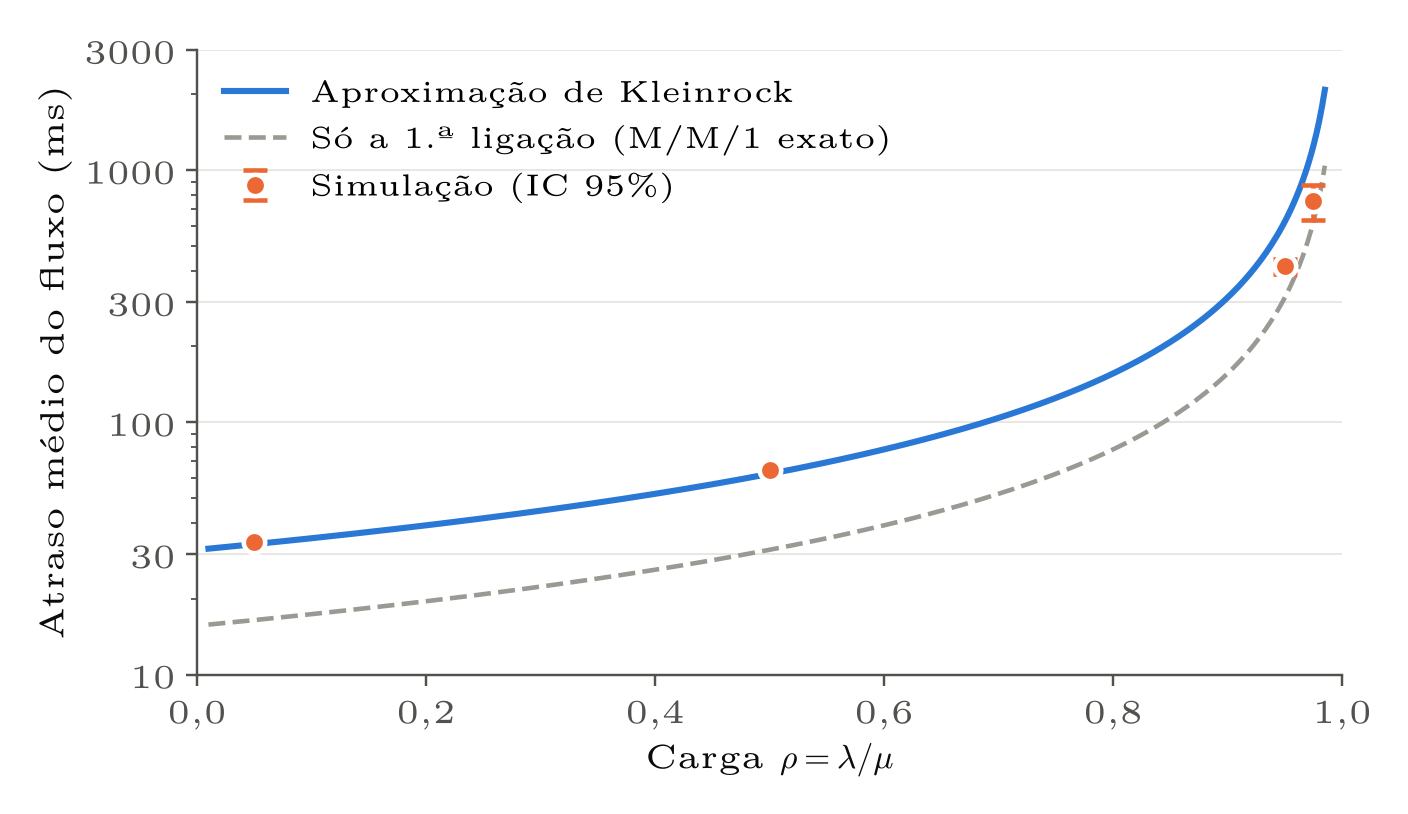
\includegraphics[width=0.75\textwidth]{figuras/ex12_kleinrock.png}
\caption{Atraso médio do fluxo em função da carga (escala logarítmica): aproximação de Kleinrock, atraso exato da primeira ligação (M/M/1) e simulação.}
\label{fig:ex12}
\end{figure}

Com carga baixa e moderada ($\rho=0{,}05$ e $0{,}5$), a aproximação de Kleinrock é muito precisa, com erros de 2\% e 3\% (Tabela~\ref{tab:ex12}). Com carga elevada sobrestima bastante o atraso: em 50\% com $\rho=0{,}95$ e em 66\% com $\rho=0{,}975$. A Figura~\ref{fig:ex12} mostra que, perto da saturação, o atraso simulado fica muito mais próximo do atraso da primeira ligação isolada do que do valor de Kleinrock.

A primeira ligação recebe chegadas de Poisson com tamanhos independentes e é exatamente uma fila M/M/1, com atraso $1/(\mu-\lambda)$. O erro está, por isso, todo na segunda ligação, que a aproximação também trata como M/M/1. Mas cada pacote mantém o tamanho que tinha na primeira ligação, e o intervalo entre duas chegadas consecutivas à segunda ligação é sempre maior ou igual ao tempo de transmissão do segundo pacote. Os tamanhos dos pacotes e os tempos entre chegadas ficam correlacionados, o que viola a hipótese M/M/1. Subtraindo ao atraso simulado o atraso exato da primeira ligação, a segunda contribui com cerca de 103~ms com $\rho=0{,}95$ e 128~ms com $\rho=0{,}975$, contra os 312,5~ms e 625~ms previstos. Com carga elevada, os pacotes chegam à segunda ligação já espaçados pela transmissão na primeira e quase não esperam. No limite de pacotes de tamanho fixo, não há espera nenhuma na segunda ligação, como se viu nos slides de redes de comutação de pacotes.

Com carga baixa, a mesma correlação tem um efeito ligeiro no sentido oposto, e a aproximação subestima o atraso em 2\% a 3\%. Um pacote curto que tenha esperado na primeira ligação por um pacote longo é transmitido logo a seguir a ele, e chega à segunda ligação enquanto o pacote longo ainda lá está a ser transmitido, pelo que volta a esperar.

Conclui-se que a aproximação de Kleinrock é precisa com carga baixa e moderada, mas com carga elevada sobrestima muito o atraso. É, nessa zona, uma aproximação conservadora: um dimensionamento baseado nela fica do lado seguro, mas com mais capacidade do que a necessária.


\newpage

% ===============================================================
% G. Redes de comutação de circuitos
% ===============================================================
\section{Redes de comutação de circuitos}

% ---------------------------------------------------------------
\subsection{Exercício 14: Dimensionamento de uma rede de comutação de circuitos}

Cada chamada ocupa $b=64$~kb/s, ou seja, um circuito, pelo que as capacidades das ligações são expressas em número de circuitos. Os três fluxos têm carga oferecida $\rho=0{,}5$~Erlang. As ligações foram identificadas pela ordem do vetor LinkCosts do \texttt{reducload\_cost.R}: L1:~1-2 (500~€ por circuito), L2:~2-3 (500~€), L3:~1-4 (100~€), L4:~2-4 (1000~€) e L5:~4-3 (100~€).

A probabilidade de bloqueio de uma ligação com $C$ circuitos e carga $\rho$ é dada pela fórmula de Erlang B (Equação~\ref{eq:erlangb}). Para o bloqueio dos fluxos foram usadas duas aproximações, ambas baseadas na hipótese de que o bloqueio é independente de ligação para ligação:
\begin{itemize}
  \item \textbf{\textit{Product bound}} (Equação~\ref{eq:prodbound}): cada ligação recebe a soma das cargas dos fluxos que a atravessam. O resultado é um limite superior do bloqueio de cada fluxo.
  \item \textbf{Aproximação de carga reduzida} (Equação~\ref{eq:reducload}): a carga que um fluxo oferece a uma ligação é reduzida pela probabilidade de a chamada ser bloqueada nas outras ligações da rota. As equações de ponto fixo são resolvidas por substituições repetidas.
\end{itemize}

\formula{ER(\rho,C)=\frac{\rho^C/C!}{\sum_{i=0}^{C}\rho^i/i!}}{Fórmula de Erlang B.}{eq:erlangb}

\formula{B_k\leq1-\prod_{j\in R_k}\bigl(1-ER(\bar\rho_j,C_j)\bigr),\qquad \bar\rho_j=\sum_{k\in K_j}\rho_k}{\textit{Product bound} ($R_k$: rota do fluxo $k$; $K_j$: fluxos que atravessam a ligação $j$).}{eq:prodbound}

\formula{L_j=ER\Bigl(\sum_{k\in K_j}\rho_k\prod_{i\in R_k-\{j\}}(1-L_i),\,C_j\Bigr),\qquad B_k\approx1-\prod_{j\in R_k}(1-L_j)}{Aproximação de carga reduzida ($L_j$: bloqueio da ligação $j$; $B_k$: bloqueio do fluxo $k$).}{eq:reducload}

\subsubsection*{a) Rotas e capacidades de custo mínimo}

Como cada chamada ocupa um circuito em todas as ligações da rota, as rotas foram escolhidas pelo custo por circuito do caminho completo. Para o fluxo 1 (1→2), a ligação direta custa 500~€, contra 1100~€ pelo caminho 1-4-2. Para o fluxo 2 (2→3), a ligação direta custa 500~€, contra 1100~€ por 2-4-3. Para o fluxo 3 (1→3), o caminho 1-4-3 custa 200~€, contra 1000~€ pelo caminho 1-2-3. Este último tem a vantagem de partilhar as ligações L1 e L2 com os outros fluxos, o que as torna mais eficientes, e por isso foi também testado.

As capacidades foram obtidas por tentativa e erro com o \texttt{reducload\_cost.R}, guiada pelos bloqueios das ligações. Começou-se com as ligações diretas e, depois, com o fluxo 3 pelo nó 4 (Tabela~\ref{tab:ex14a}).

\begin{table}[H]
\centering
\begin{tabular}{cccS[table-format=1.3]S[table-format=1.3]S[table-format=4.0]c}
\toprule
Tentativa & Rota do fluxo 3 & Circuitos em L1--L5 & {Fluxos 1 e 2 (\%)} & {Fluxo 3 (\%)} & {Custo (€)} & {$<1\%$?}\\
\midrule
1 & 1-2-3 & 4, 4, 0, 0, 0 & 1.504 & 2.985 & 4000 & não\\
2 & 1-2-3 & 5, 5, 0, 0, 0 & 0.305 & 0.609 & 5000 & sim\\
3 & 1-4-3 & 3, 3, 3, 0, 3 & 1.266 & 2.439 & 3600 & não\\
4 & 1-4-3 & 4, 4, 4, 0, 3 & 0.158 & 1.410 & 4700 & não\\
\textbf{5} & \textbf{1-4-3} & \textbf{4, 4, 4, 0, 4} & {\textbf{0,158}} & {\textbf{0,314}} & {\textbf{4\,800}} & \textbf{sim}\\
\bottomrule
\end{tabular}
\caption{Tentativa e erro com o \texttt{reducload\_cost.R} (bloqueios pela aproximação de carga reduzida). Os fluxos 1 e 2 usam sempre as ligações diretas e têm o mesmo bloqueio.}
\label{tab:ex14a}
\end{table}

Pelo caminho 1-2-3, as ligações L1 e L2 recebem 1 Erlang cada e precisam de 5 circuitos, num custo de 5000~€ (tentativas 1 e 2). Pelo caminho 1-4-3, cada ligação recebe apenas 0,5 Erlang. Com 3 circuitos o bloqueio de uma ligação é $ER(0{,}5;3)=1{,}27\%$ (tentativa 3) e com 4 circuitos é $ER(0{,}5;4)=0{,}158\%$, pelo que todas as ligações usadas precisam de 4 circuitos. A tentativa 4 mostra que não basta reforçar uma das ligações do fluxo 3. Neste caso, a partilha das ligações não compensa a diferença de preço face ao caminho via nó 4. Qualquer outra alternativa usaria a ligação L4, que é a mais cara.

\begin{figure}[H]
\centering
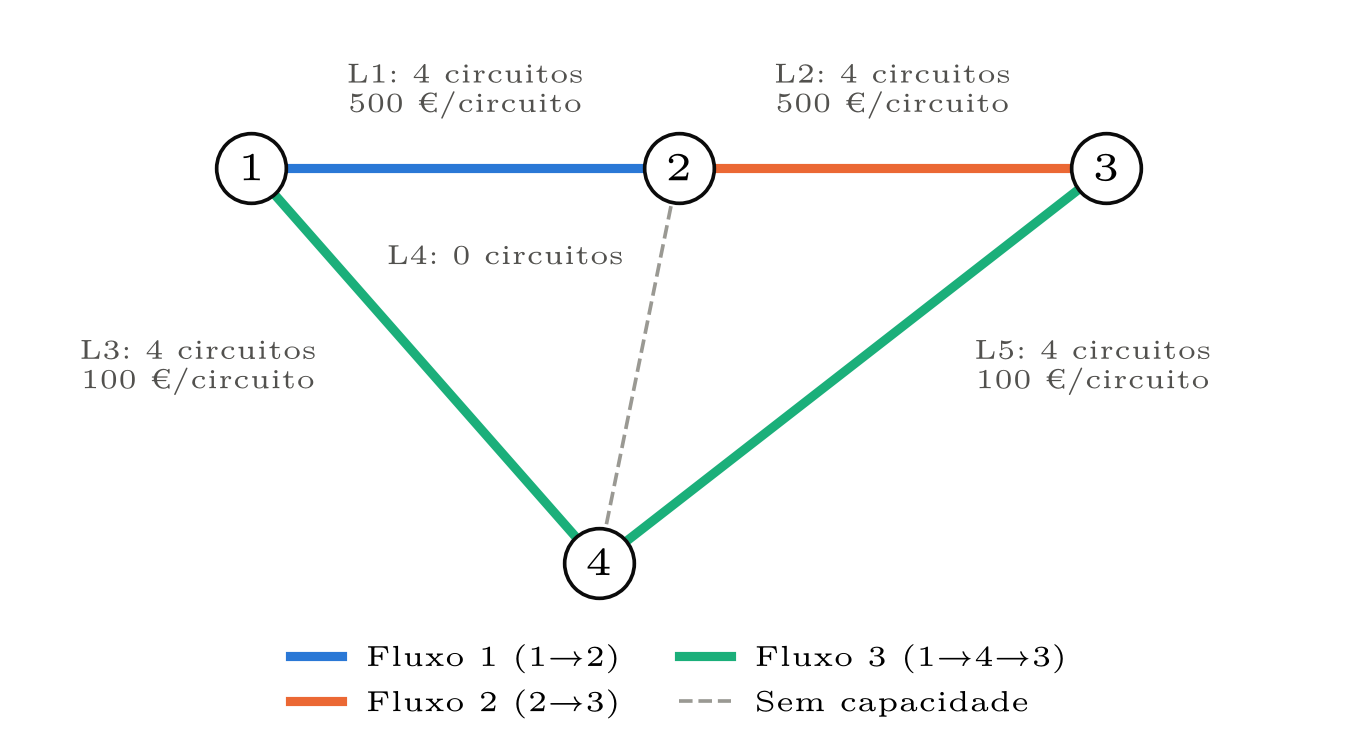
\includegraphics[width=0.7\textwidth]{figuras/ex14_rede.png}
\caption{Solução de custo mínimo: rotas dos três fluxos e capacidade instalada em cada ligação.}
\label{fig:ex14rede}
\end{figure}

A solução de custo mínimo (Figura~\ref{fig:ex14rede}) usa as rotas 1-2 para o fluxo 1, 2-3 para o fluxo 2 e 1-4-3 para o fluxo 3, com 4 circuitos (256~kb/s) nas ligações L1, L2, L3 e L5 e sem capacidade na ligação L4. O custo total é de 4800~€ e os bloqueios são de 0,158\% nos fluxos 1 e 2 e de 0,314\% no fluxo 3.

\subsubsection*{b) Validação por simulação}

A solução da alínea a) foi simulada com o simulador \texttt{cnet.R}, com as mesmas capacidades e rotas. Cada fluxo tem taxa de chegada de 0,5 chamadas por unidade de tempo e duração média unitária ($\rho=0{,}5$), e cada chamada ocupa um circuito. O tempo de simulação foi de \num{100000} unidades de tempo, o que dá cerca de \num{50000} chamadas por fluxo. Com bloqueios da ordem de 0,16\%, isto corresponde a apenas cerca de 80 chamadas bloqueadas por fluxo, pelo que não convém usar simulações mais curtas. Foram realizadas $R=10$ simulações independentes e calculado o intervalo de confiança a 95\% com a Equação~\ref{eq:ic}.

\begin{table}[H]
\centering
\begin{tabular}{cS[table-format=1.3]c}
\toprule
Fluxo & {Carga reduzida (\%)} & {Simulado (\%, IC 95\%)}\\
\midrule
1 & 0.158 & $0{,}165\pm0{,}012$\\
2 & 0.158 & $0{,}160\pm0{,}014$\\
3 & 0.314 & $0{,}151\pm0{,}012$\\
\bottomrule
\end{tabular}
\caption{Probabilidade de bloqueio de cada fluxo: aproximação de carga reduzida e simulação com o \texttt{cnet.R} (10 simulações).}
\label{tab:ex14b}
\end{table}

Nos fluxos 1 e 2, a aproximação de carga reduzida está dentro do intervalo de confiança da simulação (Tabela~\ref{tab:ex14b}). Cada um destes fluxos usa uma única ligação que não partilha com nenhum outro, e nesse caso a fórmula de Erlang B é exata. No fluxo 3, a aproximação dá cerca do dobro do bloqueio simulado. As ligações L3 e L5 são usadas apenas pelo fluxo 3, pelo que têm sempre o mesmo número de circuitos ocupados: uma chamada que encontra a ligação L3 com circuitos livres encontra também a L5. O bloqueio das duas ligações não é independente, ao contrário do que a aproximação assume, e a rota comporta-se como uma única ligação de 4 circuitos, com bloqueio exato $ER(0{,}5;4)=0{,}158\%$. Este valor está dentro do intervalo de confiança da simulação. É o caso apresentado nos slides de redes de comutação de circuitos sobre as limitações do \textit{product bound}: um único fluxo numa rota de $J$ ligações iguais tem bloqueio $ER(\rho,C)$, qualquer que seja $J$.

Os resultados da simulação são mais fiáveis, porque a simulação reproduz o funcionamento da rede sem assumir independência entre ligações. A sua única fonte de erro é estatística e está quantificada pelos intervalos de confiança. A aproximação de carga reduzida é, mesmo assim, útil no dimensionamento: o cálculo é imediato, ao contrário de uma simulação, e neste caso o erro é conservador, porque sobrestima o bloqueio.

\subsubsection*{c) \textit{Product bound}}

O bloqueio pelo \textit{product bound} foi calculado com o \texttt{prodbound.R}, com as capacidades e rotas da alínea a). A Figura~\ref{fig:ex14bloq} compara os três métodos.

\begin{table}[H]
\centering
\begin{tabular}{cS[table-format=1.4]S[table-format=1.4]}
\toprule
Fluxo & {\textit{Product bound} (\%)} & {Carga reduzida (\%)}\\
\midrule
1 & 0.1580 & 0.1580\\
2 & 0.1580 & 0.1580\\
3 & 0.3157 & 0.3140\\
\bottomrule
\end{tabular}
\caption{Probabilidade de bloqueio de cada fluxo pelo \textit{product bound} e pela aproximação de carga reduzida.}
\label{tab:ex14c}
\end{table}

\begin{figure}[H]
\centering
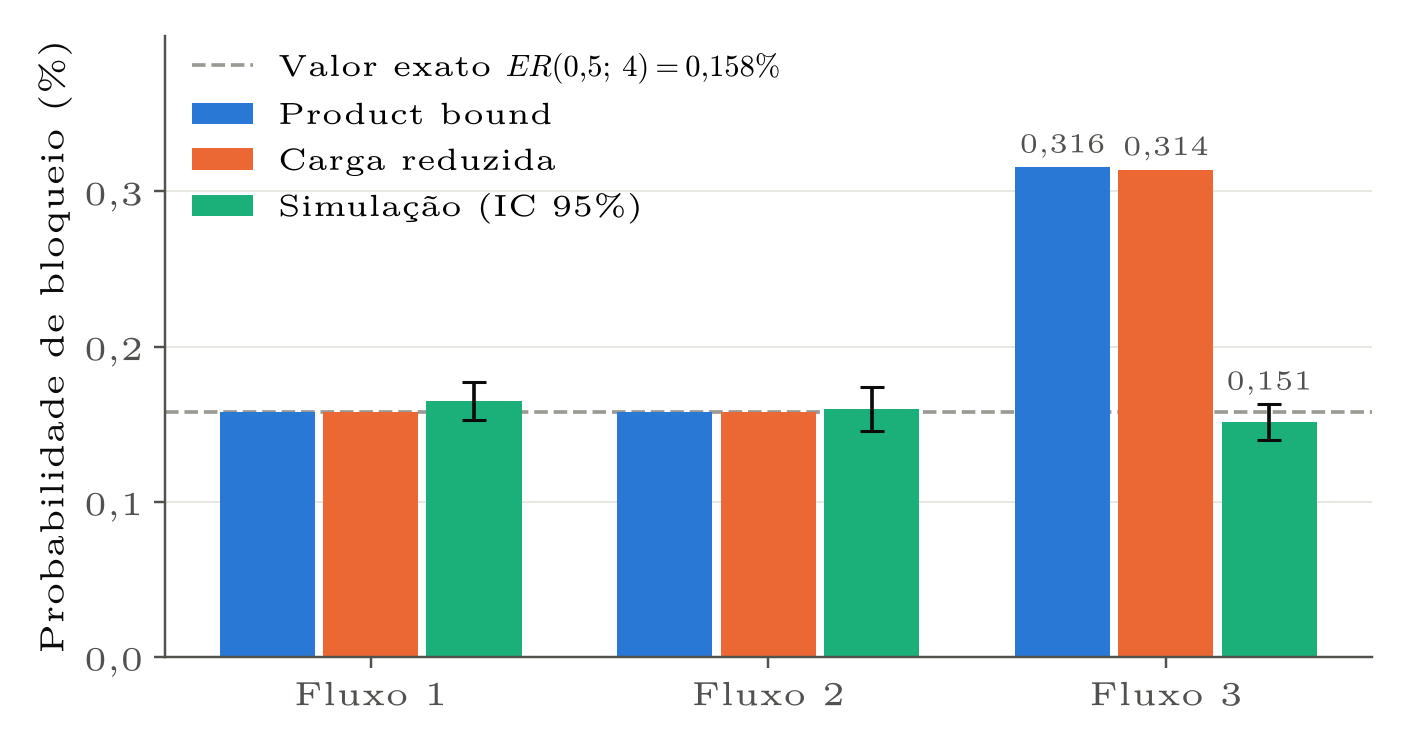
\includegraphics[width=0.75\textwidth]{figuras/ex14_bloqueio.png}
\caption{Probabilidade de bloqueio de cada fluxo pelos três métodos; a tracejado, o bloqueio exato de uma ligação de 4 circuitos com 0,5~Erlang.}
\label{fig:ex14bloq}
\end{figure}

Nos fluxos 1 e 2, o \textit{product bound} coincide com a aproximação de carga reduzida, porque numa rota de uma só ligação não há carga a reduzir (Tabela~\ref{tab:ex14c}). No fluxo 3 é ligeiramente superior (0,3157\% contra 0,3140\%), porque não desconta as chamadas bloqueadas na outra ligação da rota. Como os bloqueios são muito pequenos, essa redução quase não altera a carga, e as duas aproximações praticamente coincidem. O \textit{product bound} confirma-se como limite superior e, por não precisar de iterações, é a forma mais simples de verificar se um dimensionamento cumpre o limite de bloqueio. No entanto, partilha com a aproximação de carga reduzida a hipótese de independência entre ligações, e por isso também sobrestima o bloqueio do fluxo 3 para cerca do dobro (Figura~\ref{fig:ex14bloq}).


\newpage

% ---------------------------------------------------------------
% Referências
% ---------------------------------------------------------------
\addcontentsline{toc}{section}{Referências}
\begin{thebibliography}{10}
\bibitem{bertsekas1992} D. Bertsekas e R. Gallager, \textit{Data Networks}, 2.ª ed. Englewood Cliffs, NJ, EUA: Prentice-Hall, 1992.
\bibitem{kleinrock1975} L. Kleinrock e F. A. Tobagi, ``Packet switching in radio channels: Part I, carrier sense multiple-access modes and their throughput-delay characteristics,'' \textit{IEEE Trans. Commun.}, vol. COM-23, n.º 12, pp. 1400--1416, dez. 1975.
\bibitem{metcalfe1976} R. M. Metcalfe e D. R. Boggs, ``Ethernet: Distributed packet switching for local computer networks,'' \textit{Commun. ACM}, vol. 19, n.º 7, pp. 395--404, jul. 1976.
\bibitem{abramson1970} N. Abramson, ``The ALOHA System: Another alternative for computer communications,'' em \textit{Proc. AFIPS Fall Joint Computer Conf.}, vol. 37, 1970, pp. 281--285.
\bibitem{lorawan} LoRa Alliance, ``TS001-1.0.4 LoRaWAN L2 1.0.4 Specification,'' out. 2020.
\bibitem{ieee80211} \textit{IEEE Standard for Information Technology, Part 11: Wireless LAN Medium Access Control (MAC) and Physical Layer (PHY) Specifications}, IEEE Std 802.11-2020, 2021.
\bibitem{ieee8023} \textit{IEEE Standard for Ethernet}, IEEE Std 802.3-2022, 2022.
\bibitem{f5nginx} F5, ``What is NGINX?,'' F5 Glossary. [Online]. Disponível: \url{https://www.f5.com/glossary/nginx}. Acedido em: nov. 2026.
\bibitem{nginxdocs} F5 NGINX, ``HTTP Load Balancing,'' NGINX Documentation. [Online]. Disponível: \url{https://docs.nginx.com/nginx/admin-guide/load-balancer/http-load-balancer/}. Acedido em: nov. 2026.
\bibitem{f5lb} F5, ``Choosing an NGINX Plus Load-Balancing Technique,'' F5 Blog. [Online]. Disponível: \url{https://www.f5.com/company/blog/nginx/choosing-nginx-plus-load-balancing-techniques}. Acedido em: nov. 2026.
\end{thebibliography}


\end{document}